\chapter{Analoge Ausgänge und Eingänge}
% analogWrite: Fading von LEDs (Kerzenfunkeln mit drei gelben LEDs), dann Exkurs zur RGB Tabelle und RGB-LED revisited: fast beliebige Farben erzeugen
% Potentiometer und dimmbare Lampe; Exkurs: Nutzung des Potentiometers ohne Mikrocontroller
Digitale Bauteile haben ein Problem: Sie kennen nur Eins oder Null, An oder Aus, Wahr oder Falsch. Die Realität ist aber natürlich um einiges komplexer, nämlich analog: Reale Größen können durch im Prinzip beliebige reelle Zahlen ausgedrückt werden. Daher wäre es wünschenswert, auch analoge Werte angeben zu können. In diesem Kapitel lernst du, wie man mit dem Arduino quasi-analoge Werte erzeugen oder einlesen kann. Dabei ist es nie möglich, wirklich beliebig genaue Werte zu erreichen, wie man es bei analogen Werten erwarten würde, aber es gibt einige interessante Tricks, wie man mit einem digitalen Bauteil analoge Werte simulieren kann.

\bigskip
In diesem Kapitel lernst du\dots
\begin{itemize}
	\item \dots Pulsweitenmodulation und Hexadezimalzahlen zu benutzen,
	\item \dots Spannungen zu messen und Spannungen an einem Spannungsteiler zu berechnen,
	\item \dots logische Bedingungen mit logischen Operationen zu verfeinern,
	\item \dots ein Potentiometer, einen LDR sowie einen NTC auszulesen, um eine Drehung, die Umgebungshelligkeit bzw. die Temperatur zu messen,
	\item \dots wie Transistoren verwendet werden und was diese mit dem Aufbau des Arduino zu tun haben,
	\item \dots was es mit dem EVA-Prinzip auf sich hat.
\end{itemize}

\bigskip

\begin{projektueberblick}
	\item Kerzenfunkeln \dotfill \pageref{proj:kerzen}
	\item Farbenspektakel mit RGB-Codes \dotfill \pageref{proj:rgbled2}
	\item Batterietester (kleine Spannung) \dotfill \pageref{proj:batterietesterklein}
	\item Batterietester (große Spannung) \dotfill \pageref{proj:batterietestergross}
	\item Dimmbare Lampe \dotfill \pageref{proj:dimmlampe}
	\item Dimmbare Lampe ohne $\mu C$ \dotfill \pageref{proj:dimmlampeomc}
	\item Straßenlampe \dotfill \pageref{proj:strassenlampe}
	\item Alarmanlage \dotfill \pageref{proj:alarmanlage}
	\item Thermometer \dotfill \pageref{proj:thermometer}
\end{projektueberblick}
\newpage

\section{Pulsweitenmodulation (PWM)}\label{sec:pwm}

\begin{ziel}
	\textbf{Ziel:} Mithilfe des Arduino soll eine funkelnde LED-Kerze gebaut werden.
\end{ziel}

\begin{wrapfigure}{r}{0.35\textwidth}
	\centering
	
\includegraphics[width=0.35\textwidth]{./pics/analogwrite.png}
\end{wrapfigure}
Der Arduino verfügt über mehrere sogenannte PWM-Pins, die mit einer Tilde ($\sim$) gekennzeichnet sind. Diese lassen sich mit dem Befehl \button{setze PWM-Pin <\_> Ausgang auf <\_>} ansteuern. Im ersten Argument muss die Nummer des Pins angegeben werden, im zweiten Argument wird ein PWM-Wert zwischen 0 und 255 angegeben.

\begin{aufgabe} \emph{Fading}
	\begin{enumerate}[label=\alph*), itemsep=0ex, parsep=0ex]
		\item Schließe eine LED mit Vorwiderstand an einen PWM-Pin an und verwende die PWM-Anweisung mit unterschiedlichen PWM-Werten. Beschreibe die Wirkung auf die LED in einem Je-Desto-Satz.
		\item Lege eine Variable \button{h} für den PWM-Wert an. Nutze die Variable, um systematisch alle PWM-Werte von 0 bis 255 zu durchlaufen, sodass jeder Wert kurz sichtbar wird (z.\,B. 0.2 Sekunden).
		\item \emph{Für Schnelle:} Sorge dafür, dass die PWM-Werte nach Erreichen der 255 genauso rückwärts von 255 bis 0 durchlaufen werden.
	\end{enumerate}
\end{aufgabe}

\begin{aufgabe} \emph{Pulsweitenmodulation}
	
	Erkläre mithilfe der Zusammenfassung zur Pulsweitenmodulation, was bei der Nutzung des Befehls \button{Setze PWM-Pin 5 Ausgang auf 158} passiert. Berechne auch die mittlere Spannung, die am PWM-Pin ausgegeben wird.
	
	\emph{Für Physik-Profis:} Eine blaue LED hält bis zu 3,5\,V aus, ohne durchzubrennen. Trotzdem darf man sie bei Verwendung dieses Befehls nicht ohne Vorwiderstand an den Pin anschließen. Begründe.
	
	\emph{Für Informatik-Profis:} Wie viel Bit stehen zur Speicherung des Tastverhältnisses mit Werten von 0 bis 255 zur Verfügung?
\end{aufgabe}

\marginpar{%
	\footnotesize%
	\werkzeug Neues \\
	Werkzeug:\\
	\hyperref[sec:servo]{Servo-\\motor}%
}
\begin{projekt}[Kerzenfunkeln]\label{proj:kerzen}
	Modelliere mithilfe von drei LEDs das Funkeln von Kerzen.
	
	Tipp: Die Verwendung des Blocks für Zufallszahlen wird dir helfen, das Funkeln natürlicher aussehen zu lassen.
\end{projekt}

\newpage

\begin{zsfg}{Pulsweitenmodulation (PWM)}
	
	\begin{wrapfigure}{r}{0.45\textwidth}
		\centering
		\begin{tikzpicture}[scale=0.8]
		\fill [white] (-1.2,-1.3) rectangle (7,7.1);
		\draw [->] (0,-1) -- (0,6.5);
		\draw [->] (-1,0) -- (6.5,0);
		\draw [dashed] (4,-1) -- ++(0,7.5);
		\node at (-0.2,-0.3) {\scriptsize 0};
		\foreach \x in {1,...,6} {
			\draw (\x,0.1) -- (\x,-0.1) node [anchor=north, fill=white] {\scriptsize\x};
			\draw (0.1,\x) -- (-0.1,\x) node [anchor=east] {\scriptsize\x};
		}
		\node at (6.5,-0.35) {\scriptsize Zeit};
		\node at (0,6.5) {\parbox{1.7cm}{\scriptsize El. Potential in V}};
		\draw [thick, blue] (0,5) -- ++(1,0) ++(0,-5) -- ++(3,0) ++(0,5) -- ++(1,0) ++(0,-5) -- ++(1.5,0);
		\draw [thick, red] (0,1.25) -- ++(6.5,0) node [above] {$\overline{U}$};
		\draw [<->] (0,-0.6) -- (4,-0.6) node [below left=1mm] {\scriptsize Periodendauer T};
		\end{tikzpicture}
		\caption{Darstellung des zeitlichen Verlaufs einer Pulsweitenmodulation mit einem Tastverhältnis von 25\%.}
	\end{wrapfigure}
	Bei der Pulsweitenmodulation wechselt der ausgewählte digitale Pin sehr schnell zwischen den elektrischen Potentialen 5\,V und 0\,V hin und her - es ergibt sich also ein gepulstes Signal, dessen Weite (Dauer) moduliert werden kann. Aus dem Verhältnis der Zeit, in der der Pin auf einem 5\,V-Potential liegt, zu der Zeit, in der der Pin auf einem 0\,V-Potential liegt, ergibt sich eine mittlere Spannung (gegenüber Ground), die scheinbar am Pin anliegt. Wenn der Pin in der Hälfte der Zeit auf 5\,V und in der anderen Hälfte auf 0\,V liegt, dann ergibt sich eine mittlere Spannung von $\overline{U}=2,5\,V$. Wenn der Pin nur in einem Viertel der Zeit auf 5\,V liegt, dann ergibt sich eine mittlere Spannung von $\overline{U}=1,25\,V$ ($=5\,V\cdot 0,25$).
	
	Das Verhältnis der Zeit mit 5\,V zu der Gesamtdauer einer Periode mit 5\,V und 0\,V wird als \emph{Tastverhältnis} bezeichnet. Im Programm wird das Tastverhältnis durch einen Wert zwischen 0 und 255 angegeben. Eine 0 bedeutet, dass die Zeit mit 5\,V 0\% ausmacht, also liegt der Pin durchgängig auf einem 0\,V-Potential. Eine 255 bedeutet, dass die Zeit mit 5\,V 100\% ausmacht, also liegt der Pin durchgängig auf einem 5\,V-Potential. Diese beiden Werte entsprechen dem, was bei den bekannten Befehlen zur Steuerung von digitalen Pins passiert.
	
	Ein Wert von 100 bedeutet einen Anteil von $\frac{100}{255}\approx 0,39$ der Periodendauer. Daraus ergibt sich eine mittlere Spannung von $\overline{U}=5\,V\cdot 0,39\approx 1,96\,V$.
\end{zsfg}

\newpage
\subsection{RGB-Farben aus Hexadezimalzahlen erzeugen}\label{proj:rgbled2}

Als wir uns das erste Mal die RGB-LED angeschaut haben (siehe S. \pageref{proj:rgbled1}), war die Anzahl der Farben, die wir erzeugen konnten, noch stark limitiert. Das ändert sich mit der Möglichkeit, die Farbanteile über PWM zu dimmen. Häufig werden die Farbanteile im RGB-Modell jedoch nicht in Dezimalzahlen zwischen 0 und 255 angegeben, sondern durch Hexadezimalzahlen - z.\,B. \texttt{\#CAFF70}.

\begin{ziel}
	\textbf{Frage:} Wie kann man aus dem RGB-Hexadezimal-Code die PWM-Werte bestimmen?
\end{ziel}

\begin{aufgabe} \emph{Hexadezimalzahlen}
	\begin{enumerate}[label=\alph*), itemsep=0ex, parsep=0ex]
		\item Du kennst bereits das Dezimalsystem zur Basis 10 mit Ziffern von 0 bis 9 und das Binärsystem zur Basis 2 mit den Ziffern 0 und 1. Der RGB-Code nutzt eine Raute zu Anfang und danach das Hexadezimalsystem zur Basis 16. Wie viele Ziffern gibt es hier? Stelle anhand des Beispielcodes \texttt{\#CAFF70} eine Vermutung darüber auf, wie die Ziffern lauten.
		\item Der RGB-Code lässt sich in drei Zahlen zerlegen, die die Anteile von Rot, Grün und Blau angeben:
		\begin{equation*}
			 \# \underbrace{\texttt{CA}}_{\text{Anteil Rot~}} \underbrace{\texttt{FF}}_{\text{Anteil Grün~}} \underbrace{\texttt{70}}_{\text{Anteil Blau}}.
		\end{equation*}
		Rechne die einzelnen Zahlen vom Hexadezimalsystem ins Dezimalsystem um.
		
		\emph{Zur Erinnerung:} Im Dezimalsystem bedeutet die Zahl $70$: $7\cdot 10^1 + 0 \cdot 10^0$. Übertrage diese Zerlegung für das Hexadezimalsystem. Übersetze die Buchstabenziffern vorher ins Dezimalsystem ($\texttt{A}_{16}=10_{10},~ \texttt{B}_{16}=11_{10}, \dots$).
		\item \emph{Für Denker:} Wie viele verschiedene Farben kann man mithilfe des RGB-Farbcodes darstellen?
	\end{enumerate}
\end{aufgabe}

\begin{aufgabe} \emph{RGB-Codes}
	\begin{enumerate}[label=\alph*), itemsep=0ex, parsep=0ex]
		\item Bestimme anhand des RGB-Hexadezimal-Farbcodes die PWM-Werte für Rot, Grün und Blau in der folgenden Tabelle.
		\item Schließe eine RGB-LED mit Vorwiderstand an den Arduino an (siehe S. \pageref{proj:rgbled1}) und erzeuge nacheinander die Farben aus der Tabelle.
	\end{enumerate}
\end{aufgabe}

% die Farben für diese Tabelle sind in commands.tex mithilfe des xcolor-Pakets definiert
\begin{table}[H]
	\centering
	\begin{minipage}[c]{\textwidth}
		\begin{tabu} to \textwidth {X[L,2]X[L]X[L]|X[L,2]X[L]X[L]}
			\toprule
			\textbf{Farbe} & \textbf{Hex-Code} & \textbf{PWM-Werte} & \textbf{Farbe} & \textbf{Hex-Code} & \textbf{PWM-Werte} \\
			\midrule
			\textcolor{blueviolet}{\rule{1cm}{0.4cm}} Blue-Violet	& \texttt{\# 8A2BE2} &  & \textcolor{olivedrab}{\rule{1cm}{0.4cm}} OliveDrab & \texttt{\# 6B8E23} &  \\ 
			\textcolor{turquoise1}{\rule{1cm}{0.4cm}} Turquoise1	& \texttt{\# 00F5FF} &  & \textcolor{khaki}{\rule{1cm}{0.4cm}} Khaki & \texttt{\# F0E68C} &  \\
			\textcolor{chocolate}{\rule{1cm}{0.4cm}} Chocolate	& \texttt{\# D2691E} &  & \textcolor{deeppink}{\rule{1cm}{0.4cm}} DeepPink & \texttt{\# FF1493} &  \\
			\bottomrule
		\end{tabu}
	\end{minipage}
	\label{tab:rgb-codes}
\end{table}

\begin{projekt}[Farbenspektakel mit RGB-Farbcodes]
	Lasse die RGB-LED mithilfe des Fadings (vgl. Aufgabe \emph{Fading} zur PWM) möglichst viele Farbwerte durchlaufen und beobachte das Funkeln.
\end{projekt}
\newpage
\newgeometry{twoside, top=1cm, outer=2.6cm, inner=2.6cm, % inner und outer sind aus irgendeinem Grund vertauscht
	marginparwidth=2cm, marginparsep=0.3cm,% Die Breite für die Marginalien (Randbemerkungen) auf der rechten Seite
	bottom=1cm, footskip=24pt, %Abstand zwischen Textboden und Fußzeilenboden
	includefoot, includehead}
\begin{zsfg}{Das Hexadezimalsystem}
	
	Im Gegensatz zum Dezimalsystem zur Basis 10 mit Ziffern von 0 bis 9 und zum Binärsystem zur Basis 2 mit den Ziffern 0 und 1 arbeitet das Hexadezimalsystem mit der Basis 16 und den Ziffern 0, \dots, 9, A, B, C, D, E, F. Die Buchstaben werden als Ziffern gewählt, weil bei der üblichen 10, 11, 12, ... nicht deutlich würde, dass es sich nur um \emph{eine} Ziffer zur Basis 16 handelt.
	
	Im Hexadezimalsystem wird jede Zahl durch die Potenzen von 16 zusammengesetzt. Die Hexadezimalzahl \texttt{AF5} bedeutet dann so viel wie $\texttt{A}\cdot 16^2 + \texttt{F}\cdot 16^1 + \texttt{5}\cdot 16^0$. Den Wert der Hexadezimalzahl im Dezimalsystem erhält man dann durch eben diese Rechnung, wobei für die Buchstabenziffern die Dezimalzahlen eingesetzt werden müssen: $10\cdot 16^2 + 15\cdot 16 + 5\cdot 1 = 2805$.
	
	Da bei kleineren Ziffern wie \texttt{405} nicht ersichtlich ist, ob es sich um eine Hexadezimalzahl handeln soll, wird der Zahl häufig ein \texttt{0x} vorangestellt: \texttt{0x405}. Ebenfalls üblich ist es, die Basis im Index zu notieren: $\texttt{405}_{16}$ zeigt eine Hex-Zahl an; $405_{10}$ eine Dezimalzahl.
	
	\bigskip
	\textbf{Der RGB-Farbcode}
	
	Der RGB-Farbcode setzt jede Farbe aus Rot, Grün und Blau zusammen, wobei jede Farbe einen unterschiedlichen Anteil an der Mischung haben kann. Der Anteil wird durch eine Zahl zwischen 0 und 255 ausgedrückt; es steht für jede Farbe also ein Byte (acht Bit) zur Verfügung.
	
	Es wäre allerdings umständlich und für Menschen schlecht lesbar, für jede Farbe acht Nullen bzw. Einsen zu notieren. Die entsprechenden Dezimalzahlen wären zwar schon übersichtlicher, jedoch lassen sich Dezimalzahlen von digitalen Bauteilen schlechter verarbeiten, weil die 10 keine Zweierpotenz ist. Die Basis 16 schafft hier Abhilfe: Als vierte Potenz von Zwei ($16=2^4$) lassen sich die Ziffern zur Basis 16 durch genau vier Bit darstellen. Zum Beispiel ist $13_{10}=\texttt{D}_{16}=1101_2$. Zweistellige Hex-Zahlen lassen sich dann durch acht Bit, also ein Byte darstellen. Der Wertebereich reicht von \texttt{00} (also 0) bis \texttt{FF} (also $15\cdot 16 + 15 \cdot 1=255$) und passt damit genau zum RGB-Farbraum.
	
	\begin{wrapfigure}{r}{0.45\textwidth}
		\centering
		%\vspace{-1.5\baselineskip}
		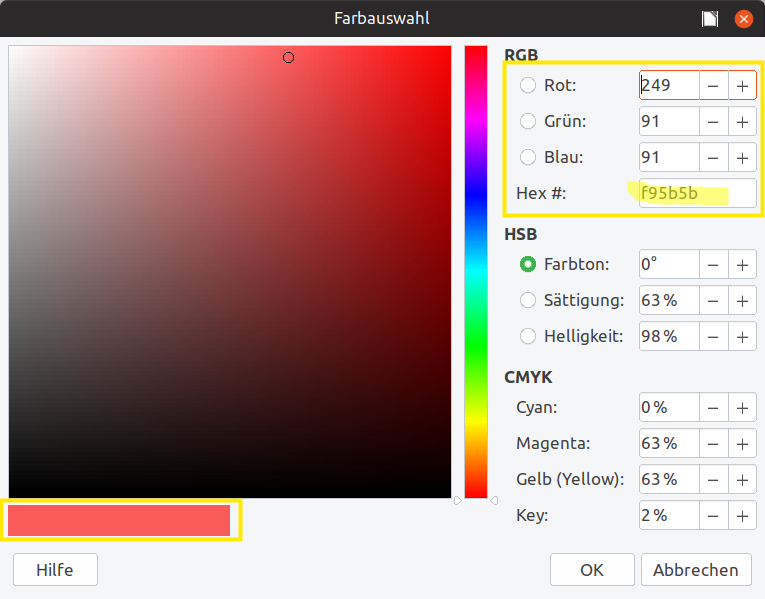
\includegraphics[width=0.45\textwidth]{./pics/Farbauswahl-LibreOffice.png}
		\caption{RGB-Farbcode in LibreOffice (rechts oben; die Angabe erfolgt über Dezimalzahlen oder Hexzahlen).}
		%\vspace{-1\baselineskip}
	\end{wrapfigure}
	Um deutlich zu machen, dass die folgenden Hex-Zahlen eine Farbe im RGB-Code codieren, wird den drei Hex-Zahlen für die drei Farbanteile eine Raute vorangestellt. Aus den insgesamt sechs Ziffern, für die jeweils 16 mögliche Werte existieren, ergeben sich $16^6=16777216$ verschiedene Farben, die sich codieren lassen. Das sind mehr Farben als das menschliche Auge unterscheiden kann.
	
	RGB-Farbcodes werden in zahlreichen Programmen wie zum Beispiel der Textverarbeitung LibreOffice genutzt (siehe Abbildung rechts). Im Internet findet man zudem \href{http://www.farb-tabelle.de/de/farbtabelle.htm}{Farbtabellen mit der Angabe der Codes}.
\end{zsfg}
\restoregeometry
\onehalfspacing

\section{Spannung messen an analogen Eingängen}

Wenn Batterien kaum noch Ladung gespeichert haben, lässt die Spannung an ihren Polen nach und sinkt unter den Wert, der auf der Batterie vermerkt ist. Mithilfe der analogen Eingänge A0 bis A5 lässt sich die Spannung messen und so entscheiden, ob die Batterie noch brauchbar ist.
\marginpar{%
	\textattachfile[description={Arbeitsblatt zu Kap. \thechapter, Spannung messen}]{./Auftraege/kap5-batterietester.pdf}{
	\footnotesize%
	\drucker Vorlage%
	}%
	\footnotesize%
	%\drucker \href{run:./Auftraege/kap5-batterietester.pdf}{Vorlage}
	\\öffnen%
}

\begin{ziel}
	\textbf{Frage:} Wie kann man mit dem Arduino eine Spannung messen?
\end{ziel}

\marginpar{%
	\scriptsize%
	\ausrufezeichen Achtung: \\
	Ganze Zahlen:\\
	10/1023 \\
	= 0 \\
	Kommazahlen:\\
	10/1023.0 \\
	= 0.01
}
\begin{projekt}[Batterietester (Voltmeter für $U<5\,V$)]\label{proj:batterietesterklein}
	\begin{wrapfigure}{r}{0.3\textwidth}
		\centering
		\begin{tabular}{c | c}
			\textbf{Analogwert} & \textbf{Spannung} \\ \hline
			0 & 0\,V \\ \hline
			1 &  \\ \hline
			100 &  \\ \hline
			1023 & 5\,V \\ \hline
		\end{tabular}
	\end{wrapfigure}
	Für eine einfache Messung bei einer 1,5\,V-Batterie wird der negative Pol der Batterie mit GND verbunden, sodass ein gemeinsames Nullpotential vorliegt. Der positive Pol der Batterie wird mit einem der analogen Eingänge A0 bis A5 verbunden. Über einen eingebauten Analog-Digital-Wandler (\emph{engl. analog-to-digital converter, ADC}) wird der Spannungswert durch eine Zahl zwischen 0 und 1023 ausgedrückt.
	 
	\begin{enumerate}[label=\alph*), itemsep=0mm, parsep=0mm]
	 	\item Schließe eine mit 1,5\,V beschriftete Batterie an den Arduino an und miss die Spannung. Berechne aus dem Analogwert die Spannung und lass sie auf dem seriellen Monitor ausgeben.
	 	\item Ergänze den Batterietester um eine Ampel, die anzeigt, ob die Batterie voll aufgeladen bzw. noch in Ordnung bzw. leer ist.
	 	\item \emph{Für Informatik-Profis:} Wie viel Bit Speicherplatz werden für den Analogwert zwischen 0 und 1023 gebraucht?
	\end{enumerate}	
\end{projekt}
%\footnotesize Achtung: Das Programm rechnet 100/1023 = 0 (Division ganzer Zahlen mit Abrundung), 100/1023.0 = 0.0978 (Division von Gleitkommazahlen).

%\normalsize

\begin{projekt}[Batterietester (Voltmeter für $U>5\,V$)]\label{proj:batterietestergross}
	Da der Arduino beim direkten Anschließen nur maximal 5\,V \enquote{verträgt}, muss man zum Testen von z.\,B. 9\,V-Blöcken weitere Bauteile verwenden. Mit zwei $\SI{10}{\kilo\ohm}$ Widerständen kann man einen einfachen \emph{Spannungsteiler} aufbauen, der die Messung ermöglicht.
	%\vspace{-\baselineskip}
	\begin{minipage}{\textwidth}
		\begin{minipage}{0.48\textwidth}
			\begin{enumerate}[label=\alph*), itemsep=0mm, parsep=0mm]
				\item Berechne die Stromstärke und die Spannung an den Widerständen. Warum sind große Widerstände hier sinnvoll?
				\item Markiere die Kabel in der Abbildung farbig, sodass die Kabel, die auf dem gleichen elektrischen Potential liegen, die gleiche Farbe haben. Notiere zudem den Wert des elektrischen Potentials.
			\end{enumerate}
		\end{minipage}
		\hfill
		\begin{minipage}{0.48\textwidth}
			\centering
			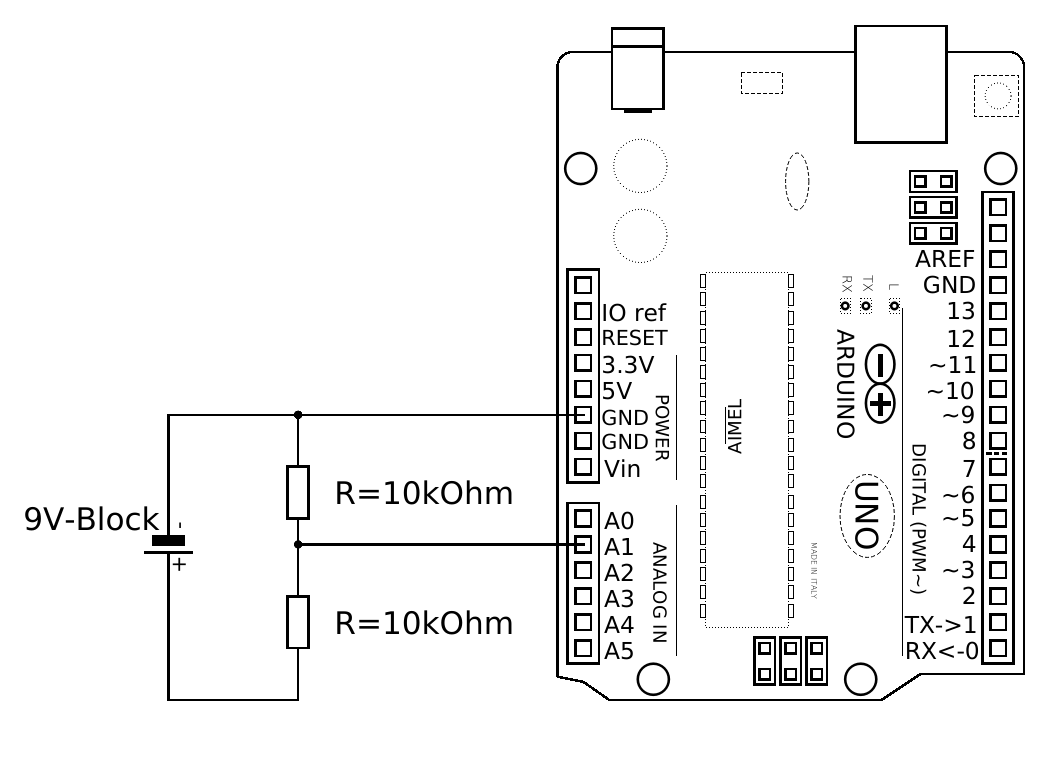
\includegraphics[width=0.95\textwidth]{./Zeichnungen/schaltplan-batterietester.png}
		\end{minipage}
	\end{minipage}
	\begin{enumerate}[label=\alph*), itemsep=0mm, parsep=0mm,start=3]
		\item Gib an, wie man mit dem Arduino die Spannung am 9\,V-Block berechnet. Baue den Batterietester dann auf und probiere ihn mit dem 9\,V-Block aus der Box aus.
		\item \emph{Zum Nachdenken:} Wie groß darf die Spannung beim oben verwendeten Spannungsteiler maximal sein, damit am Arduino nicht mehr als 5\,V anliegen? Wie könnte man den Spannungsteiler bauen, sodass man Spannungen bis zu 15\,V messen kann?
	\end{enumerate}
\end{projekt}

% Hinweis: Ganz ähnlich funktioniert ein Multimeter, bei dem man verschiedene Bereiche zum Messen der Spannung einstellen kann! Auch dort werden die Messwiderstände möglichst groß gehalten, um den Strom durch das Messgerät möglichst klein zu halten.
% Zusammenfassung: Spannung messen am Arduino und Spannungsteiler?!

\subsection{Bedingungen durch logische Operationen verfeinern}
% Beim Bau der Batterieampel kann man die und Verknüpfung verwenden -> Aufhänger zum Betrachten von kombinierten Wahrheitswerten
\marginpar{%
	\textattachfile[description={Folie zu Kap. \thechapter, Logische Operationen}]{./Auftraege/kap5-batterieampel-wahrheitswerte.pdf}{%
		\folie\footnotesize Folie%
	}%
	\footnotesize%
	%\folie \href{run:./Auftraege/kap5-batterieampel-wahrheitswerte.pdf}{Folie} \\
	\\öffnen
}
Beim Bau der Batterieampel kann die Verknüpfung von Wahrheitswerten hilfreich sein. Dazu dienen die Blöcke für die logischen Operationen \button{und}, \button{oder} und \button{nicht}, die aus zwei Bedingungen, die jeweils wahr oder falsch sein können, einen zusammenfassenden Wahrheitswert (wahr/falsch) machen bzw. den Wahrheitswert umkehren (\enquote{NICHT}).

\begin{ziel}
	\textbf{Frage:} Wie ermittelt man das Ergebnis der logischen Operationen NICHT, UND, ODER?
\end{ziel}

\begin{aufgabe} \emph{Genau draufgeschaut: Batterieampel}
	
	Wenn man die Batterieampel mit logischen Operationen realisiert, braucht man eine Bedingung der folgenden Art:
	\begin{equation*}
		spannung > 1,2\,V \quad \text{UND} \quad  spannung < 1,4\,V \quad  \text{ODER} \quad spannung = 1,4\,V
	\end{equation*}
	
	Dies lässt sich bei mBlock auf zwei Arten realisieren, die sich in der Reihenfolge der Auswertung unterscheiden (siehe Abbildung).
	
	\begin{figure}[H]
		\centering
		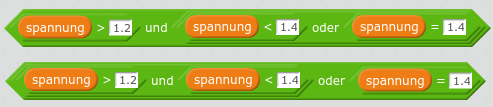
\includegraphics[width=0.6\textwidth]{./pics/batterieampel-log-operationen.png}
	\end{figure}

	Sind beide Varianten geeignet?
	
	Zur Klärung dieser Frage eignen sich in einfachen Fällen \textbf{Wahrheitswerttabellen}, die einen Überblick über das Ergebnis der logischen Operationen bieten (siehe unten). Vergleiche die beiden Varianten mithilfe von Wahrheitswerttabellen.
	
	\bigskip
	\textbf{Variante 1:}
	
	\medskip
	\begin{minipage}{\textwidth}
		\small
		\centering
		\begin{tabular}{c|c|c|c|c|c}
			U>1,2\,V & U<1,4\,V & U=1,4\,V & U<1,4\,V ODER U=1,4\,V & \parbox{4cm}{U>1,2\,V UND (U<1,4\,V ODER U=1,4\,V)} & Bemerkung\\ \hline
			1 & 1 & 1 & 1 & 1 & phys. unmögl. \\
			0 & 1 & 1 & 1 & \dots & \dots\\
			\dots & \dots & \dots & \dots & \dots & \dots\\
		\end{tabular}
	\end{minipage}
	
	\bigskip
	\textbf{Variante 2:}
	
	\medskip
	\begin{minipage}{\textwidth}
		\small
		\centering
		\begin{tabular}{c|c|c|c|c|c}
			U>1,2\,V & U<1,4\,V & U=1,4\,V & U>1,2\,V UND U<1,4\,V & \parbox{4cm}{(U>1,2\,V UND U<1,4\,V) ODER U=1,4\,V} & Bemerkung\\ \hline
			1 & 1 & 1 & 1 & 1 & phys. unmögl. \\
			0 & 1 & 1 & 0 & \dots & \dots \\
			\dots & \dots & \dots & \dots & \dots & \dots\\
		\end{tabular}
	\end{minipage}
\end{aufgabe}

\begin{minipage}{0.75\textwidth}
	\begin{aufgabe} \emph{Juke-Box 2.0}
			
		Logische Operationen lassen sich nutzen, um die Juke-Box aus Kapitel 2 zu erweitern, ohne Hardware nachrüsten zu müssen. Zur Erinnerung: Es wurden zwei Taster und ein Piezo-Summer an den Arduino angeschlossen. Wenn Taster 1 gedrückt wurde, gibt der Befehl \button{lese digitalen Pin taster1} TRUE zurück und es wurde ein entsprechender Song gespielt.
		
		Die Idee: Man kann auch beide Taster gleichzeitig oder gar keinen Taster drücken, sodass sich vier Fälle für vier Songs ergeben. Sinnvollerweise wird nur irgendeine Standardmusik gespielt, wenn gar kein Taster gedrückt wurde.
		
		Formuliere für jeden der vier Fälle eine trennscharfe Bedingung!
	\end{aufgabe}
\end{minipage}
\hfill
\begin{minipage}{0.23\textwidth}
	\centering
	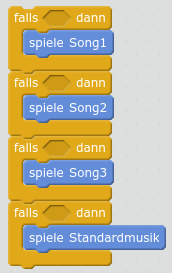
\includegraphics[width=0.98\textwidth]{./pics/jukebox2-0-leer.png}
\end{minipage}
\marginpar{%
	\textattachfile[description={Arbeitsblatt zu Kap. \thechapter, De Morgan}]{./Auftraege/kap5-wahrheitswerte-de-morgan.pdf}{%
		\ausrufezeichen
	}
	\footnotesize%
	%\ausrufezeichen \href{run:./Auftraege/kap5-wahrheitswerte-de-morgan.pdf}{De Morgan}
	De Morgan
}


\begin{zsfg}{Logische Operationen und Wahrheitswerttabellen}
	
	Logische Operationen dienen zum Verknüpfen von Wahrheitswerten - ganz so wie Rechenoperationen zum Verknüpfen von Zahlen dienen. Wir betrachten die logischen Operationen UND (AND), ODER (OR) sowie NICHT (NOT). Das Ergebnis dieser Operationen lässt sich anhand von Wahrheitswerttabellen übersichtlich festhalten. Darin wird festgehalten, ob zwei Aussagen bzw. Bedingungen A und B wahr (1) oder falsch (0) sind. In der rechten Spalte steht dann, ob die logische Operation wahr (1) oder falsch (0) ergibt.
	
	\medskip
	\begin{minipage}{0.3\textwidth}
		\centering
		\begin{tabular}{c | c | c}
			\textbf{A} & \textbf{B} & \textbf{A UND B} \\ \hline
			1 & 1 & 1 \\
			1 & 0 & 0 \\
			0 & 1 & 0 \\
			0 & 0 & 0 \\  
		\end{tabular}
	\end{minipage}
	\hfill
	\begin{minipage}{0.3\textwidth}
		\centering
		\begin{tabular}{c | c | c}
			\textbf{A} & \textbf{B} & \textbf{A ODER B} \\ \hline
			1 & 1 & 1 \\
			1 & 0 & 1 \\
			0 & 1 & 1 \\
			0 & 0 & 0 \\  
		\end{tabular}
	\end{minipage}
	\hfill
	\begin{minipage}[t]{0.3\textwidth}
		\centering
		\begin{tabular}{c | c}
			\textbf{A}  & \textbf{NICHT A} \\ \hline
			1 & 0 \\
			0 & 1 \\  
		\end{tabular}
	\end{minipage}
	
	\medskip
	Achtung: Die ODER-Operation ergibt auch dann \enquote{wahr}, wenn beide Aussagen wahr sind. Das aus dem Alltag bekannte \enquote{ENTWEDER-ODER} (XOR) ist eine weitere logische Operation, die \enquote{falsch} ergibt, wenn beide Aussagen wahr sind. Diese Operation ist aber nicht in mBlock enthalten.
\end{zsfg}

\newpage
\newgeometry{twoside, top=2cm, outer=2.6cm, inner=2.6cm, % inner und outer sind aus irgendeinem Grund vertauscht
	marginparwidth=2cm, marginparsep=0.3cm,% Die Breite für die Marginalien (Randbemerkungen) auf der rechten Seite
	bottom=1cm, footskip=24pt, %Abstand zwischen Textboden und Fußzeilenboden
	includefoot, includehead}
\section{Die Verwendung eines Potentiometers (Drehreglers)} \label{sec:potentiometer}
% Bleistiftpoti
Die Messung einer variablen, (quasi-)analogen Spannung eröffnet neue Möglichkeiten, da die Eingabewerte nun viel differenzierter sind als bei einem Taster, bei dem die Eingabe nur aus \enquote{0} oder \enquote{1} bestand. Zum Beispiel kann man darüber angeben, wie hell eine Lampe leuchten soll bzw. wie stark sie gedimmt werden soll. Dazu werden Potentiometer verwendet.

\begin{ziel}
	\textbf{Frage:} Wie funktioniert ein Potentiometer?
\end{ziel}
\marginpar{%
	\textattachfile[description={Folie zu Kap. \thechapter, Bleistiftpotentiometer}]{./Auftraege/kap5-bleistiftpoti.pdf}{%
		\footnotesize\folie Folie%
	}
	\footnotesize%
	%\folie \href{run:./Auftraege/kap5-bleistiftpoti.pdf}{Folie} \\
	\\öffnen%
}
\vspace{-1\baselineskip}
\begin{aufgabe}\emph{Bleistiftpotentiometer}
	
	\begin{minipage}{0.6\textwidth}
		\smallskip
		Ein einfaches Potentiometer kannst du selbst bauen. 
		
		\smallskip
		\emph{Basteln:} Markiere dafür mit Bleistift einen dicken Strich auf einem Blatt Papier und klebe am einen Ende ein Kabel fest, das mit GND verbunden ist. Klebe ans andere Ende ein Kabel, das mit 5V verbunden ist. Mit einem dritten Kabel (\enquote{Sensorkabel}), das mit einem analogen Eingang verbunden ist, lässt sich nun messen, welches elektrische Potential an einer beliebigen Stelle des Bleistiftstreifens anliegt.
		
		\smallskip
		\emph{Experimentieren:}	Schreibe ein Programm, dass dir fortlaufend auf dem seriellen Monitor die Analogwerte und die umgerechneten Werte für das elektrische Potenzial bzw. die Spannung gegenüber GND anzeigt. Bewege dann das Sensorkabel über den Streifen und beobachte, wie sich die Spannungswerte verändern.
	\end{minipage}
	\hfill
	\begin{minipage}{0.39\textwidth}
		\centering
		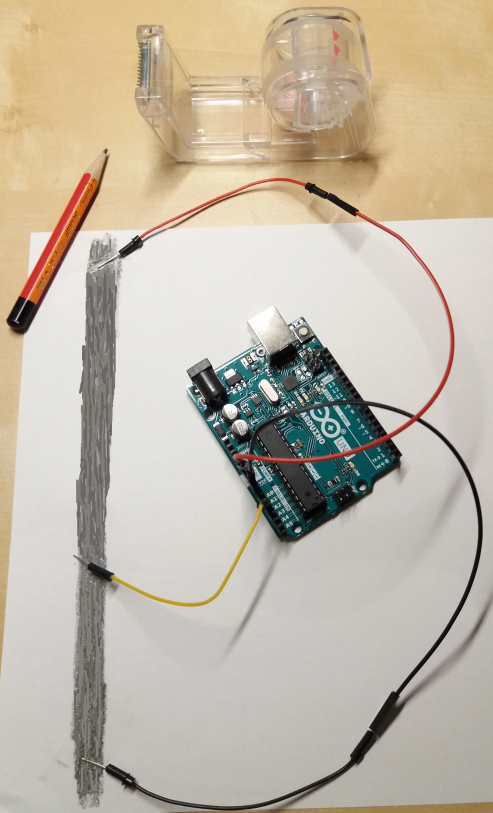
\includegraphics[width=0.75\textwidth]{./pics/bleistiftpoti-klein.png}
	\end{minipage}

	\medskip
	\emph{Analysieren:}	Der Bleistiftstreifen leitet den Strom bei einem bestimmten Gesamtwiderstand $R_{ges}$. Durch das Sensorkabel wird der Streifen in zwei Teile mit den Teilwiderständen $R_1$ und $R_2$ geteilt. Erläutere anhand deiner Beobachtungen, wie die drei Widerstände zusammenhängen.
	
	{\scriptsize Idee: Frick, Fritsch und Trick (2015): \emph{Einführung in Mikrocontroller - Der Arduino als Steuerzentrale}, Bad Saulgau}
\end{aufgabe}

\begin{zsfg}{Potentiometer}
	\begin{minipage}{0.7\textwidth}
		Ein \textbf{Potentiometer}, kurz: Poti, ist im Grunde nichts anderes als ein Spannungsteiler mit zwei Widerständen. Jedoch kann die Größe der Widerstände z.\,B. durch Drehen variiert werden. Der Gesamtwiderstand bleibt dabei immer gleich.
	\end{minipage}
	\hfill
	\begin{minipage}{0.28\textwidth}
		\begin{minipage}{0.48\textwidth}
			\centering
			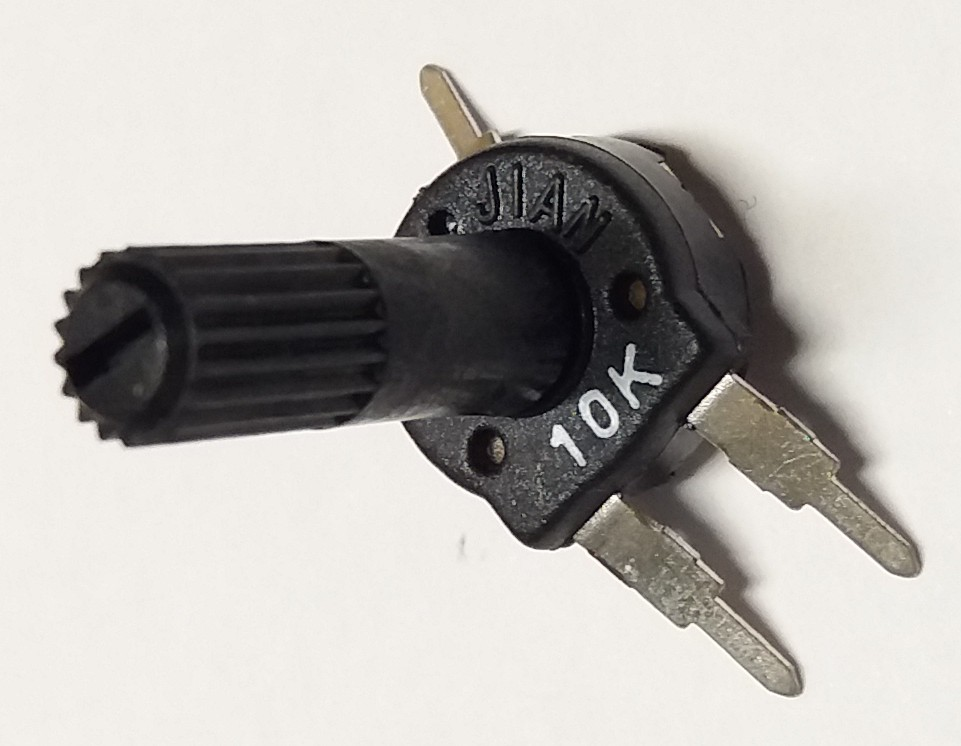
\includegraphics[angle=-90,width=0.8\textwidth]{./pics/poti.jpg}
		\end{minipage}
		\hfill
		\begin{minipage}{0.48\textwidth}
			\centering
			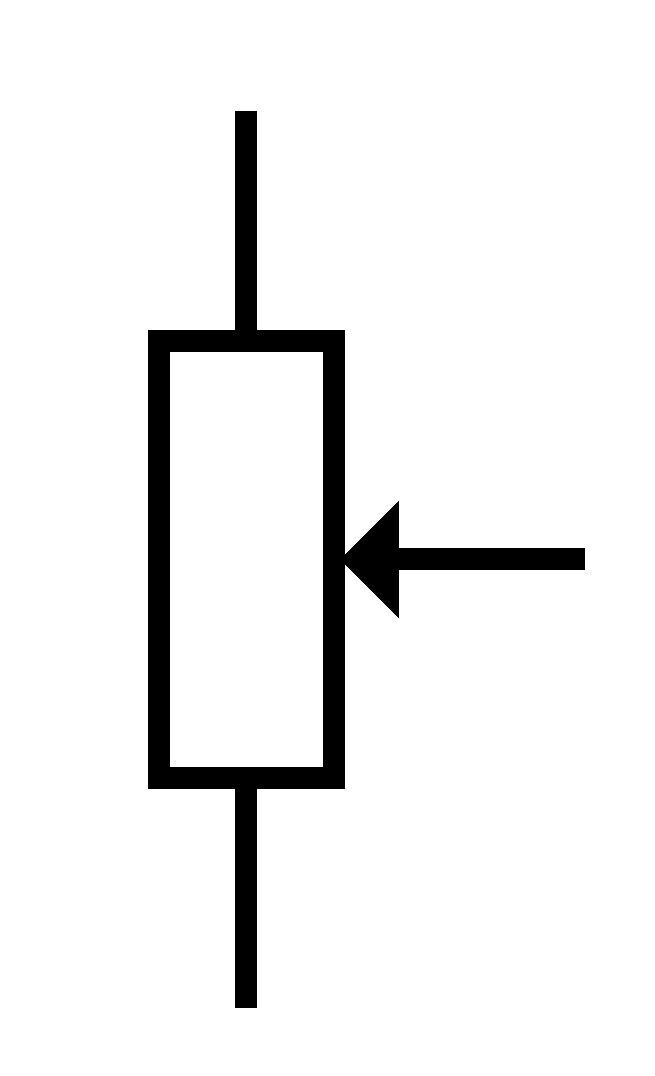
\includegraphics[width=0.65\textwidth]{./pics/poti-schaltsymbol.png}
		\end{minipage}
	\end{minipage}
	
	\smallskip
	Beim Anschluss an den Arduino wird der mittlere Pin des Potentiometers an einen analogen Eingang angeschlossen. Die anderen beiden Pins werden mit GND und 5V verbunden.
\end{zsfg}

\marginpar{%
	\footnotesize%
	\werkzeug Neues \\
	Werkzeug:\\
	\hyperref[sec:joystick]{Joystick}%
}
\begin{projekt}[Dimmbare Lampe]\label{proj:dimmlampe}
	Baue und programmiere eine Lampe, deren Helligkeit sich durch ein Potentiometer einstellen lässt.
	
	\begin{minipage}{0.8\textwidth}
		\emph{Hinweis:} Du musst dafür sorgen, dass der eingelesene Analogwert zwischen 0 und 1023 in einen PWM-Wert zwischen 0 und 255 umgerechnet wird. Ermittle dazu eine passende Funktion.
	\end{minipage}
	\hfill
	\begin{minipage}{0.19\textwidth}
		\centering
		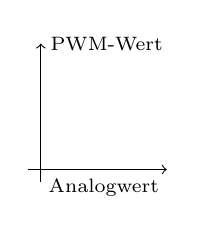
\begin{tikzpicture}[scale=0.8]
			\draw [->] (-0.2,0) -- (2,0);
			\draw [->] (0,-0.2) -- (0,2);
			\node at (1,0) [below] {\scriptsize Analogwert};
			\node at (0,2) [right] {\scriptsize PWM-Wert};
		\end{tikzpicture}
	\end{minipage}
\end{projekt}
\restoregeometry
\onehalfspacing

\subsection{Die Verwendung eines Potentiometers ohne Mikrocontroller}

Für einige Projekte, wie das Dimmen einer Lampe, ist ein Mikrocontroller eigentlich überdimensioniert, weil sich die Funktion schon durch eine reine Hardwarelösung erreichen lässt.

\begin{ziel}
	\textbf{Frage:} Wie lässt sich eine Lampe ohne Mikrocontroller dimmen?
\end{ziel}

\begin{figure}[H]
	\centering
	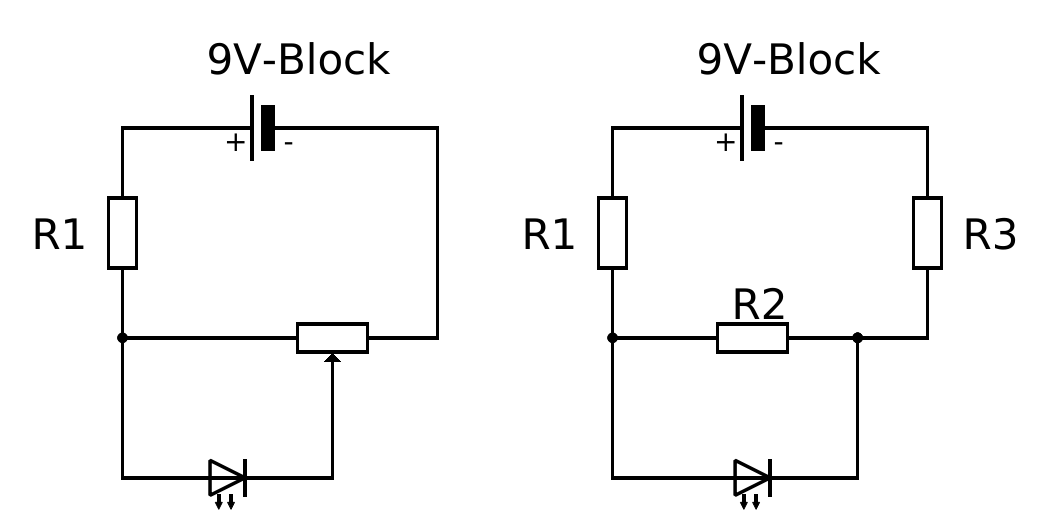
\includegraphics[width=0.6\textwidth]{./Zeichnungen/potentiometer-anwendung.png}
	\caption{Auf der linken Seite ist die Anwendung eines Potentiometers ohne Mikrocontroller dargestellt. Auf der rechten Seite ist der zugehörige Ersatzschaltplan gezeichnet, der zeigt, dass das Potentiometer als Spannungsteiler mit zwei variablen Widerständen $R_2$ und $R_3$ aufgefasst werden kann.}
\end{figure}

\begin{projekt}[Dimmbare Lampe ohne Mikrocontroller]\label{proj:dimmlampeomc}
	\vspace{-0.5\baselineskip}
	\begin{enumerate}[label=\alph*), itemsep=0mm, parsep=0mm]
		\item Erkläre, wie sich die LED verhält, wenn das Potentiometer so gedreht ist, dass gilt:
		\begin{enumerate}[label=(\arabic*), itemsep=0mm, parsep=0mm]
			\item \dots $R_2=\SI{0}{\ohm}, \quad R_3=\SI{10}{\kilo\ohm}$,
			\item \dots $R_2=\SI{10}{\kilo\ohm}, \quad R_3=\SI{0}{\ohm}$.
		\end{enumerate} 
		\item Bevor die Schaltung aufgebaut werden kann, muss die Größe des Vorwiderstands $R_1$ berechnet werden. Der Vorwiderstand muss den Strom auch dann noch klein genug halten, wenn das Potentiometer so gedreht ist, dass gilt: $R_3=\SI{0}{\ohm}$ (und dementsprechend $R_2=\SI{10}{\kilo\ohm}$).
		
		Berechne $R_1$ so, dass die Stromstärke durch die LED maximal $\SI{20}{\milli\ampere}$ beträgt.
		
		\emph{Hinweis:} Die Stromstärke durch $R_2$ kann vernachlässigt werden, sodass $I_{ges}\approx I_{LED} = \SI{20}{\milli\ampere}$ mit $U_{LED}=\SI{2,3}{\volt}$ gilt.
		
		\emph{Begründung:} Wenn $R_1=\SI{0}{\ohm}$ wäre, würde die komplette Spannung an $R_2$ abfallen. Dann gilt: $I_{R_2}=\frac{\SI{9}{\volt}}{\SI{10}{\kilo\ohm}}=\SI{0,9}{\milli\ampere}$. Die Stromstärke durch $R_2$ beträgt also nur etwa 1/20 der Stromstärke durch die LED und wenn $R_1$ größer wird, dann wird die Stromstärke durch $R_2$ sogar noch kleiner. 
		
		\item Baue die Schaltung auf und beobachte das Leuchtverhalten der LED beim Drehen am Potentiometer.
	\end{enumerate}
\end{projekt}

\newpage
Beim Experimentieren mit dem Potentiometer wirst du feststellen, dass man das Potentiometer nicht vollständig zur Seite drehen muss, damit die LED aufhört zu leuchten. Im Experiment zeigt sich, dass eine blaue LED schon bei $R_2=\SI{2,5}{\kilo\ohm}$ und $R_3=\SI{7,5}{\kilo\ohm}$ aufhört zu leuchten. Die Spannung an der LED beträgt dann $U_{L,blau}=\SI{2,3}{\volt}$.

\begin{aufgabe} \emph{Kennlinien von Leuchtdioden}
	\begin{enumerate}[label=\alph*), itemsep=0mm, parsep=0mm]
		\item Baue eine blaue LED in den oben dargestellten Schaltkreis und drehe das Potentiometer so, dass die blaue LED gerade nicht mehr leuchtet. Die Spannung an der blauen LED beträgt dann $U_{L,blau}=\SI{2,3}{\volt}$. Ersetze dann die blaue LED durch eine grüne/gelbe/rote LED. Notiere deine Beobachtungen.
		\item Ordne die Farben der LEDs den rechts abgebildeten Kennlinien von einer blauen, einer grünen, einer gelben und einer roten LED zu. Experimentiere dazu mit dem Potentiometer und den LEDs.
		
		\emph{Hinweis:} Das menschliche Auge ist in der Lage, bereits bei einer Stromstärke von wenigen Mikroampere ein schwaches Leuchten zu erkennen. Im Diagramm ist so eine geringe Stromstärke kaum von $\SI{0}{\milli\ampere}$ zu unterscheiden.
	\end{enumerate}

	\begin{figure}[H]
		\centering
		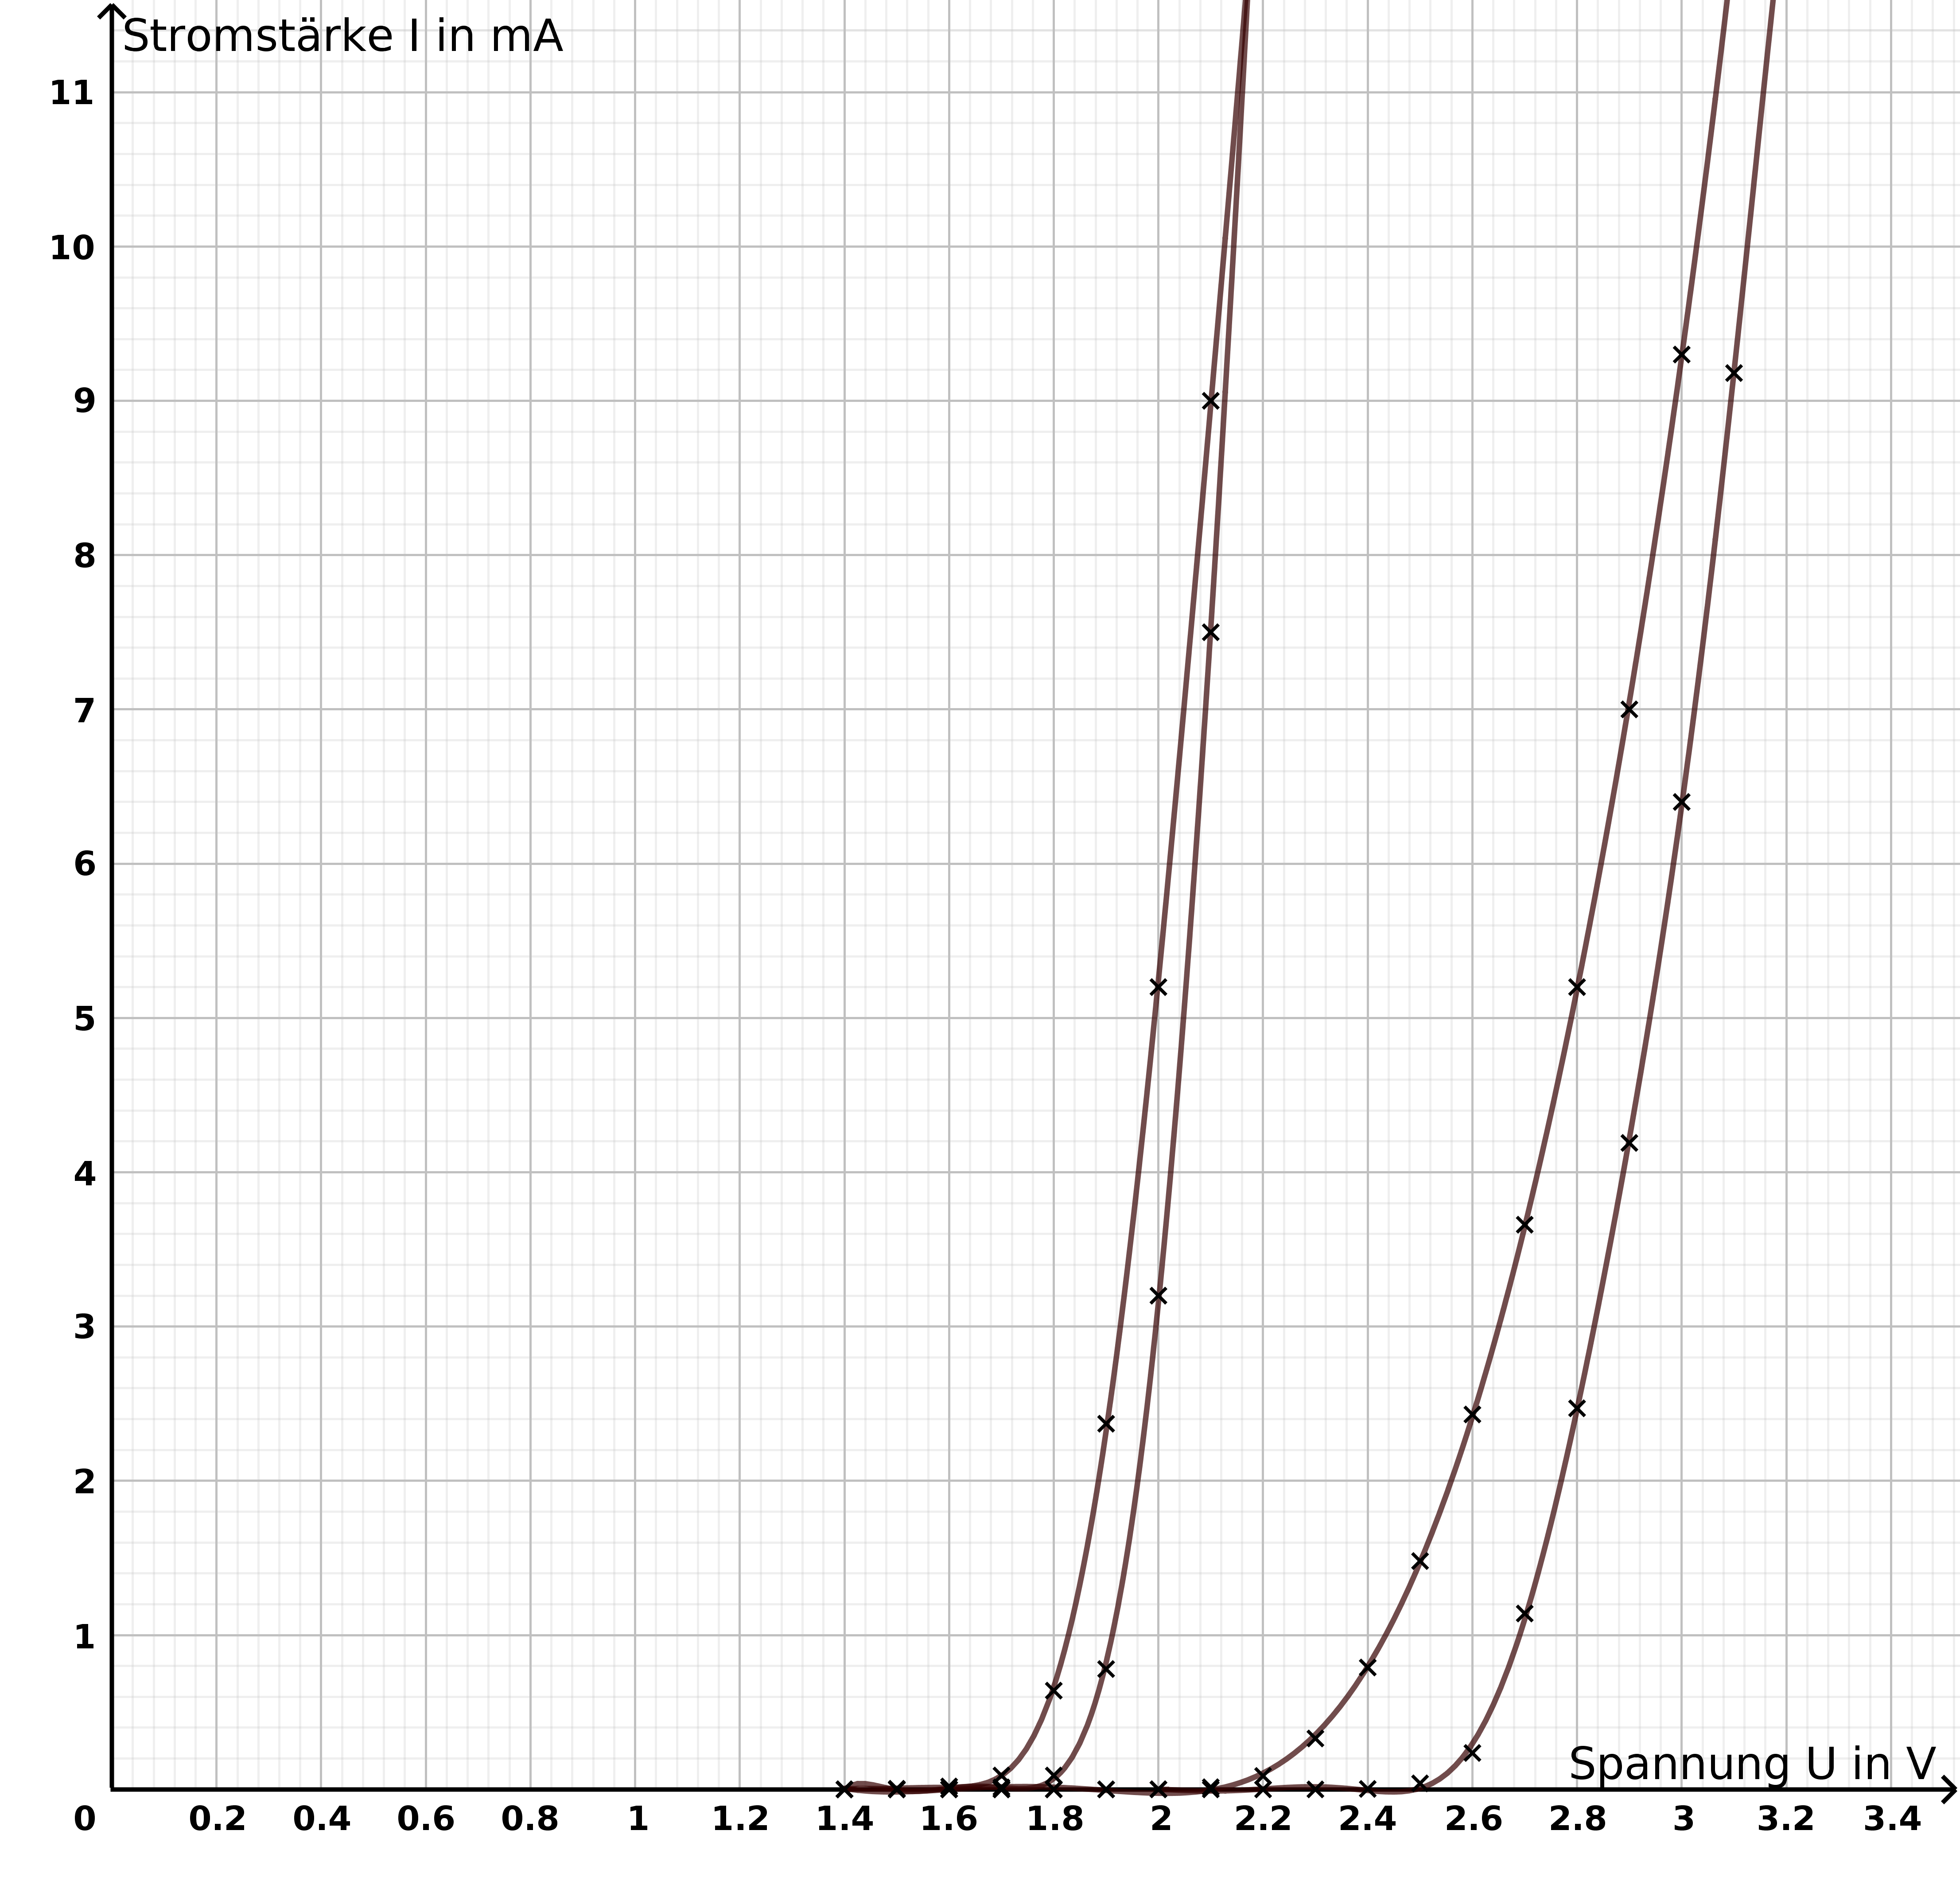
\includegraphics[width=0.85\textwidth]{./Zeichnungen/Diodenkennlinien.png}
		\caption{U-I-Kennlinien einer roten, gelben, grünen und blauen Leuchtdiode.}
	\end{figure}
\end{aufgabe}
\vfill

\section{Helligkeit messen}\label{sec:ldr}

Die Helligkeit bestimmt unseren Tages- und Jahresrhythmus: Wenn es dunkel wird, schlafen wir (oder gehen feiern) und wenn es hell wird, stehen wir wieder auf und unternehmen etwas. Es ist daher nur logisch, dass es einige Anwendungen für elektrische Schaltungen gibt, die auf die Helligkeit reagieren.\footnote{Natürlich lässt er sich auch für Spielereien nutzen. Der Author hat mit einigen LDR ein \href{https://www.el-voss.de/?p=159}{Moorhuhn-Lasertag} gebaut\dots} In einfachen Fällen wird dabei auf einen Fotowiderstand, kurz: LDR (\emph{engl. \textbf{l}ight \textbf{d}ependent \textbf{r}esistor}), zurückgegriffen.

\begin{ziel}
	\textbf{Frage:} Wie verwendet man einen Fotowiderstand/LDR am Arduino?
\end{ziel}

\begin{minipage}{0.84\textwidth}
	\begin{aufgabe}\emph{Erste Experimente mit dem LDR}
		\vspace{-0.3\baselineskip}
		\begin{enumerate}[label=\alph*), itemsep=0ex, parsep=0mm]
			\item Baue mit dem Arduino einen Spannungsteiler mit einem LDR und einem Festwiderstand von $R_1=\SI{10}{\kilo\ohm}$ so auf, dass du die Spannung am LDR in A0 messen kannst. Lasse dir die Spannung am LDR auf dem seriellen Monitor ausgeben.
			\item Beschreibe, wie sich die Spannung am LDR verhält, wenn es dunkel bzw. wenn es hell wird.
		\end{enumerate}
	\end{aufgabe}
\end{minipage}
\hfill
\begin{minipage}{0.14\textwidth}
		\centering
		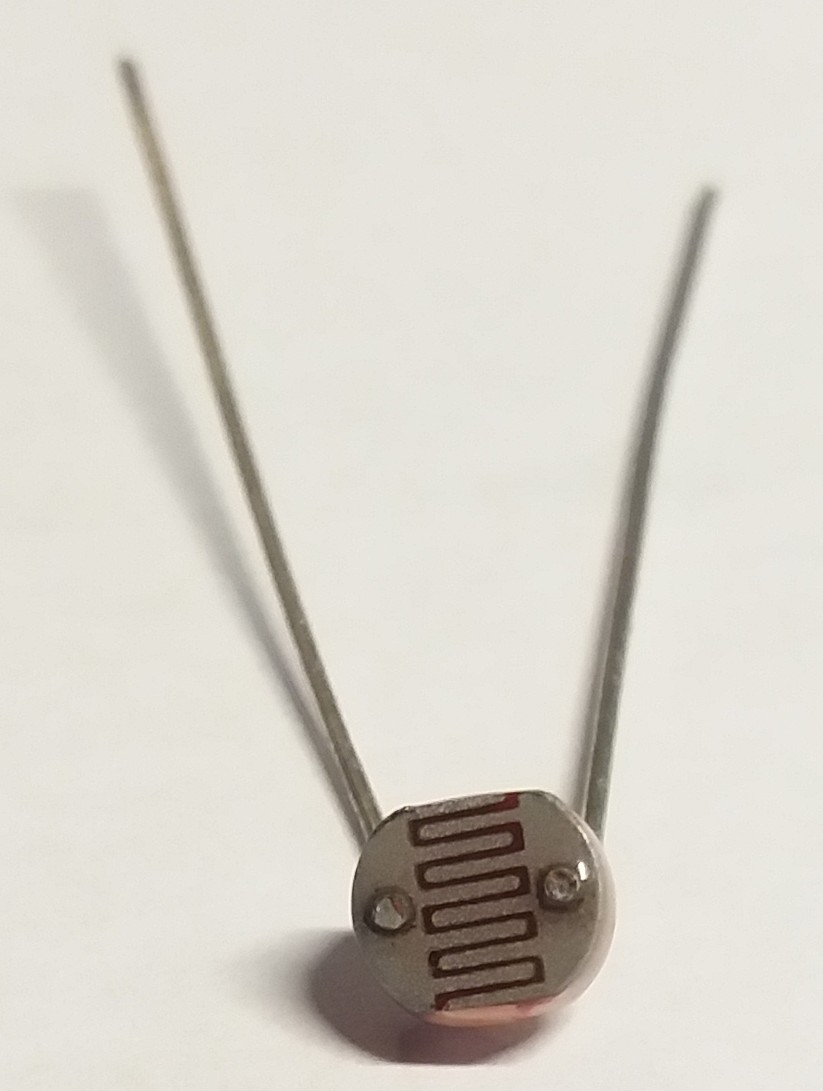
\includegraphics[width=0.9\textwidth]{./pics/ldr.jpg}
\end{minipage}

\begin{aufgabe} \emph{Genaue Analyse des Spannungsteilers}
	
	Die Änderung der Spannung resultiert aus der Änderung des Widerstands des LDR. Um einen Eindruck vom Wertebereich des Widerstands eines LDR zu bekommen, soll dieser nun berechnet werden.\medskip
	
	\begin{minipage}{0.78\textwidth}
		\begin{enumerate}[label=\alph*), itemsep=0ex, parsep=0mm]
			\item Leite eine Formel für den Spannungsteiler her, mit der du den Widerstand $R_2$ des LDR mithilfe der Spannung $U_2$ am LDR, dem Festwiderstand $R_1$ und der Spannung $U_1$ am Festwiderstand berechnen kannst.
			
			Tipp: Betrachte zuerst die Stromstärken $I_1$ und $I_2$ durch den Festwiderstand und den LDR. Durch das Sensorkabel fließt (näherungsweise) kein Strom.
			\item Berechne, welchen Widerstand der LDR hat, wenn er komplett abgedunkelt ist und wenn er mit einer Smartphone-Taschenlampe bestrahlt wird.
		\end{enumerate}
	\end{minipage}
	\hfill
	\begin{minipage}{0.2\textwidth}
		\centering
		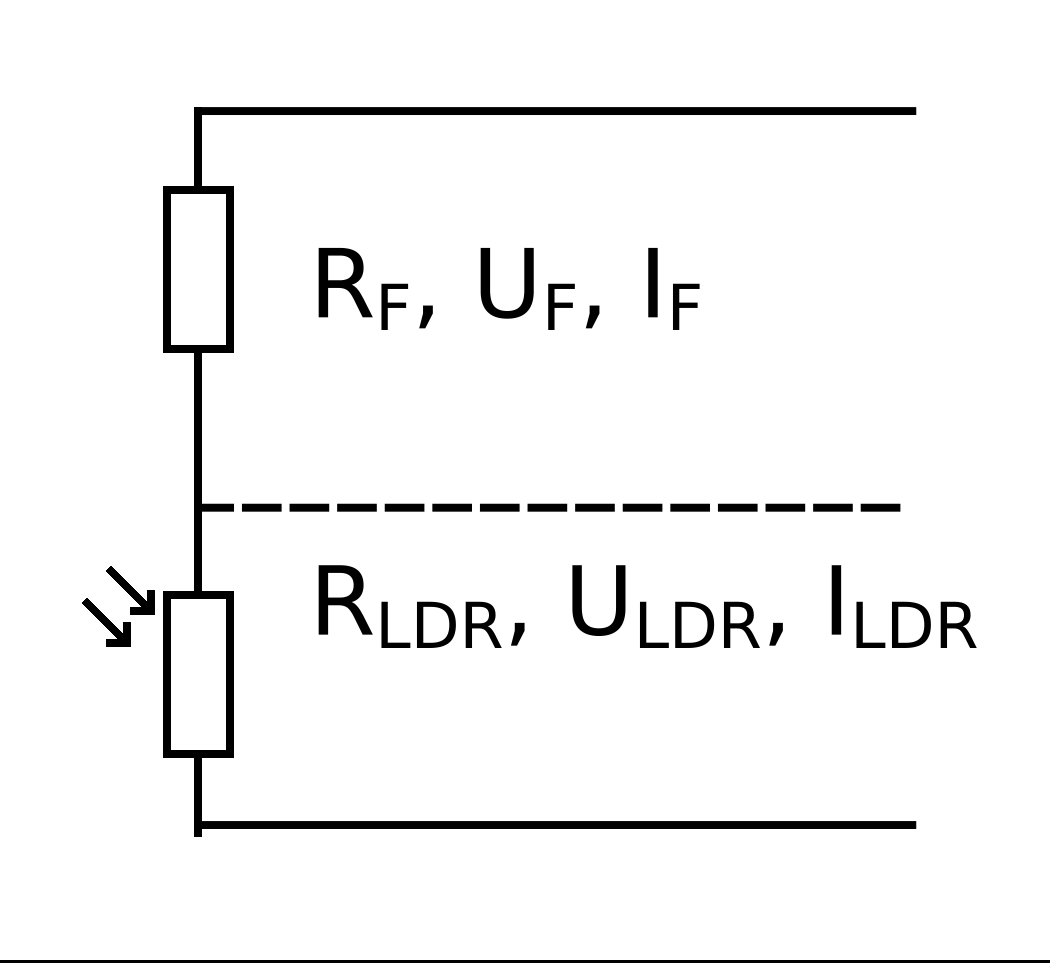
\includegraphics[width=\textwidth]{./Zeichnungen/spannungsteiler-ldr.png}
	\end{minipage}
\end{aufgabe}

%Qualitative Projekte
\begin{projekt}[Straßenlampe]\label{proj:strassenlampe}
	Baue eine Straßenlampe, deren Licht (Vorwiderstand!) angeht, wenn es dunkel wird, und ausgeht, wenn es hell wird.
\end{projekt}

\begin{projekt}[Alarmanlage mit Lichtschranke]\label{proj:alarmanlage}
	\begin{minipage}{0.78\textwidth}
		Baue eine Alarmanlage, indem du mit einer LED (Vorwiderstand!) und einem LDR eine Lichtschranke baust. Wird diese unterbrochen, soll ein akustischer Alarm ertönen.
	\end{minipage}
	\hfill
	\begin{minipage}{0.2\textwidth}
		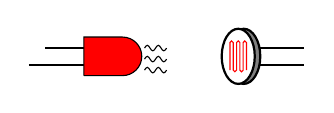
\begin{tikzpicture}[scale=0.7]
		%LED
		\draw [thick] (0,0) -- (1,0);
		\draw [thick] (0.3,0.3) -- (1,0.3);
		\draw [fill=red] (1,-0.2) -- (1,0.5) -- (1.7,0.5) arc [start angle=90,end angle=-90,radius=0.35] -- (1,-0.2);
		%Lichtstrahlen
		\draw (2.1,-0.1) sin ++(0.05,0.05) cos ++(0.05,-0.05) sin ++(0.05,-0.05) cos ++(0.05,0.05) sin ++(0.05,0.05) cos ++(0.05,-0.05) sin ++(0.05,-0.05) cos ++(0.05,0.05);
		\draw (2.1,0.1) sin ++(0.05,0.05) cos ++(0.05,-0.05) sin ++(0.05,-0.05) cos ++(0.05,0.05) sin ++(0.05,0.05) cos ++(0.05,-0.05) sin ++(0.05,-0.05) cos ++(0.05,0.05);
		\draw (2.1,0.3) sin ++(0.05,0.05) cos ++(0.05,-0.05) sin ++(0.05,-0.05) cos ++(0.05,0.05) sin ++(0.05,0.05) cos ++(0.05,-0.05) sin ++(0.05,-0.05) cos ++(0.05,0.05);
		% LDR
		\draw [thick] (4,0) -- (5,0);
		\draw [thick] (4,0.3) -- (5,0.3);
		\draw [thick,fill=gray] (3.9,0.15) ellipse [x radius=0.3,y radius=0.5];
		\draw [thick,fill=white] (3.8,0.15) ellipse [x radius=0.3,y radius=0.5];
		\draw [red] (3.65,-0.1) -- ++(0,0.5) arc [start angle=-180,end angle=-360,radius=0.03] -- ++(0,-0.5) arc [start angle=-180,end angle=0,radius=0.03] -- ++(0,0.5) arc [start angle=-180,end angle=-360,radius=0.03] -- ++(0,-0.5) arc [start angle=-180,end angle=0,radius=0.03] -- ++(0,0.5) arc [start angle=-180,end angle=-360,radius=0.03] -- ++(0,-0.5);
		\end{tikzpicture}
	\end{minipage}
\end{projekt}

\newpage
%\newgeometry{twoside, top=2cm, outer=2.6cm, inner=2.6cm, % inner und outer sind aus irgendeinem Grund vertauscht
%	marginparwidth=2cm, marginparsep=0.3cm,% Die Breite für die Marginalien (Randbemerkungen) auf der rechten Seite
%	bottom=1cm, footskip=24pt, %Abstand zwischen Textboden und Fußzeilenboden
%	includefoot, includehead}
%\onehalfspacing
%Infokasten: LDR als elektronisches Bauteil, das seinen Widerstand in Abhängigkeit der Helligkeit ändert (mit Bild und Schaltsymbol)
\begin{zsfg}{Fotowiderstand}
	\begin{minipage}{0.7\textwidth}
		Ein \textbf{Fotowiderstand}, kurz: \textbf{LDR} (\emph{engl. \textbf{l}ight \textbf{d}ependent \textbf{r}esistor}), ist ein lichtabhängiger Widerstand. Wenn es dunkel wird, wird der elektrische Widerstand des LDR größer; wenn es hell wird, wird der elektrische Widerstand des LDR kleiner.
	\end{minipage}
	\hfill
	\begin{minipage}{0.28\textwidth}
		\begin{minipage}{0.48\textwidth}
			\centering
			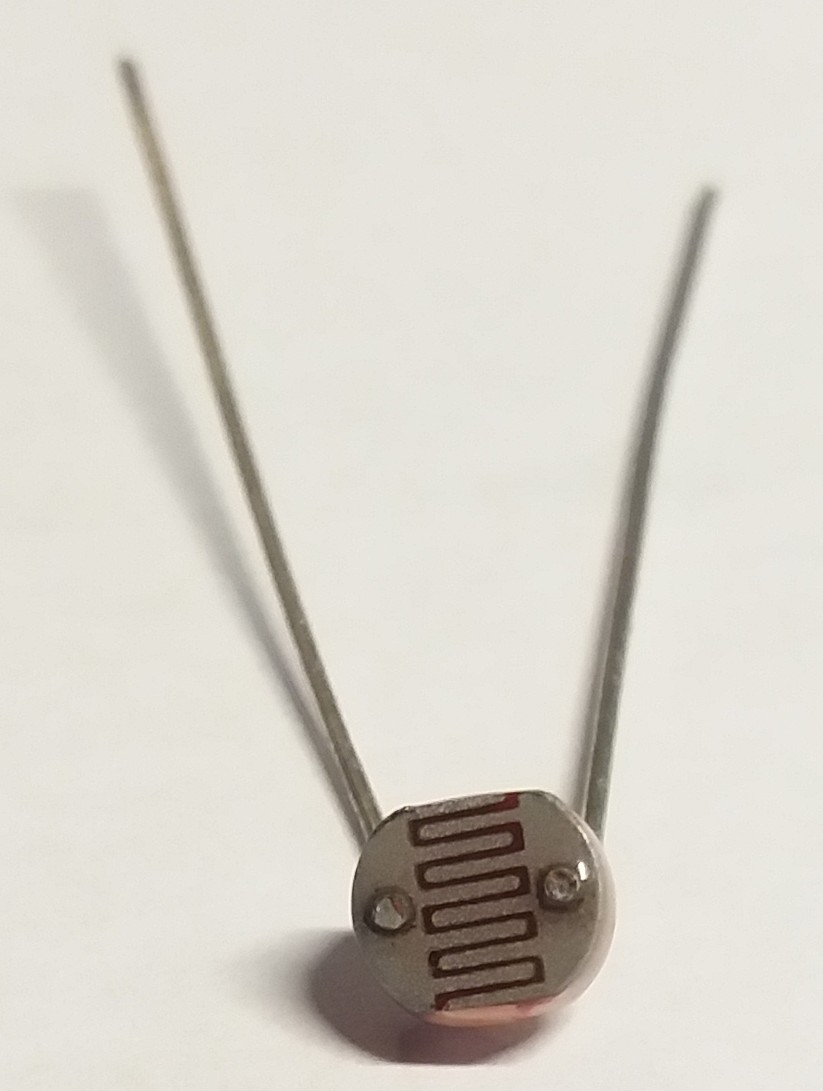
\includegraphics[width=0.9\textwidth]{./pics/ldr.jpg}
		\end{minipage}
		\hfill
		\begin{minipage}{0.48\textwidth}
			\centering
			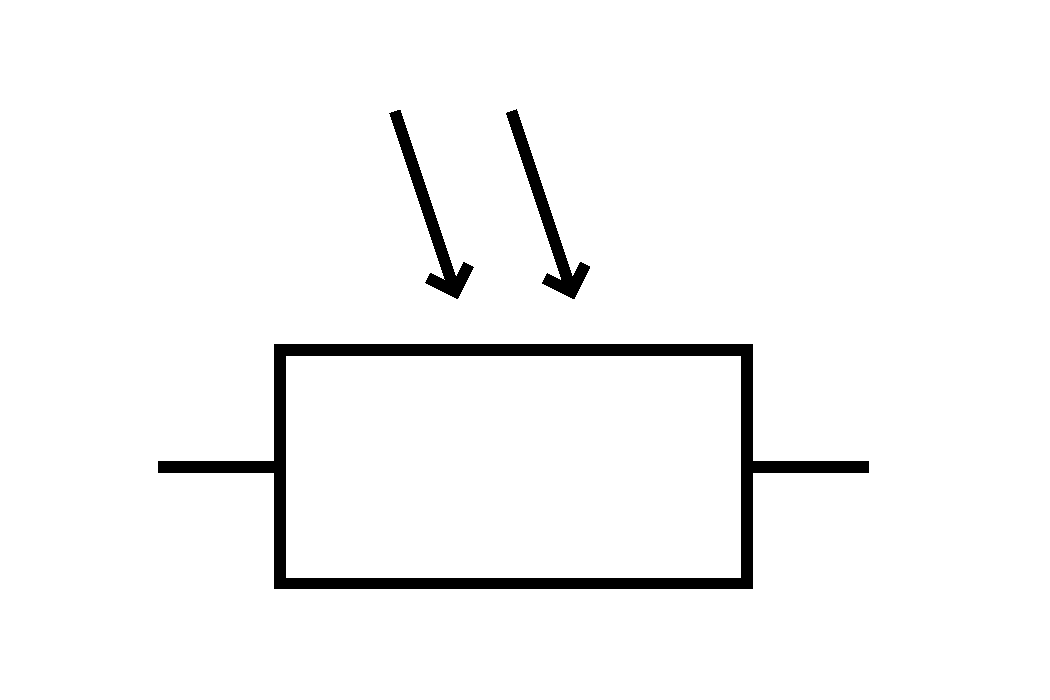
\includegraphics[width=\textwidth]{./pics/ldr-schaltsymbol.png}
		\end{minipage}
	\end{minipage}
%	\bigskip
%	\emph{Kurze Hintergrundinformation:}
%	
%	Der Fotowiderstand besteht aus einem Halbleitermaterial, in dem die Elektronen wie üblich an den Atomkern gebunden sind. Bei Halbleitern reicht jedoch schon relativ wenig Energie, um einige Elektronen so weit aus ihrer Bindung zu lösen, dass sie zum elektrischen Strom beitragen. Diese Energiezufuhr stammt von dem Licht, das auf den LDR fällt.
\end{zsfg}
%TODO: Hintergrundinfo ausführlicher - Bändermodell

Wenn man die Helligkeit wie bisher über eine Spannung messen kann, kann man schon einige interessante Projekte umsetzen. Es wäre jedoch unbefriedigend, wenn man nicht auch die Helligkeit an sich berechnen könnte. Dies kann man zum Beispiel für eine Wetterstation nutzen.

\begin{ziel}
	\textbf{Frage:} Wie kann man aus dem Widerstand des LDR die Helligkeit berechnen?
\end{ziel}

Der Zusammenhang zwischen Widerstand des LDR und der Umgebungshelligkeit ließe sich zwar theoretisch herleiten, aber das würde an dieser Stelle zu weit führen. Wir können die Formel zur Berechnung der Umgebungshelligkeit auch experimentell gewinnen. Ein erster Ansatz dazu wäre ein kontrolliertes Experiment, in dem der Widerstand des LDR bei definierter Umgebungshelligkeit gemessen wird. Leider bräuchten wir zur Festlegung der Umgebungshelligkeit aber bereits ein Messgerät für die Helligkeit. Daher entnehmen wir die zusammengehörigen Messwerte von Widerstand und Helligkeit nicht einem Experiment, sondern dem Datenblatt des LDR. Ein Datenblatt enthält in tabellarischer und oft graphischer Form die wesentlichen Kenndaten eines Bauteils. Es ist zu jedem Bauteil kostenlos im Internet zu finden.

\begin{aufgabe} \emph{Datenblatt lesen}
	
	Suche im \href{https://components101.com/sites/default/files/component_datasheet/LDR%20Datasheet.pdf}{Datenblatt des LDR}
	den Graphen, der den Zusammenhang von Helligkeit in der Einheit Lux und Widerstand des LDR in der Einheit $\SI{}{\kilo\ohm}$ abbildet. Entnimm dem Graphen fünf zusammengehörige Werte von Helligkeit und Widerstand und halte diese tabellarisch fest.
	
	\smallskip
	\begin{minipage}{0.78\textwidth}
		\emph{Achtung:} Die Achsen im Graphen sind logarithmisch skaliert. Das bedeutet, dass die Werte an den Achsen nicht gleichmäßig zunehmen, sondern exponentiell (von 0,1 zu 1 zu 10 zu 100 zu 1000). Diese Skalierung ermöglicht erst das Ablesen der Werte, aber es muss berücksichtigt werden, dass die Werte nur sehr ungenau abzulesen sind.
	\end{minipage}
	\hfill
	\begin{minipage}{0.2\textwidth}
		\begin{tikzpicture}
			\draw [->] (-0.2,0) -- (2.2,0);
			\draw [->] (0,-0.2) -- (0,2.2);
			\draw (0.5,0.1) -- ++(0,-0.2) node [below] {\tiny 0.1};
			\draw (1,0.1) -- ++(0,-0.2) node [below] {\tiny 1};
			\draw (1.5,0.1) -- ++(0,-0.2) node [below] {\tiny 10};
			\draw (2,0.1) -- ++(0,-0.2) node [below] {\tiny 100};
			\draw (0.1,0.5) -- ++(-0.2,0) node [left] {\tiny 0.1};
			\draw (0.1,1) -- ++(-0.2,0) node [left] {\tiny 1};
			\draw (0.1,1.5) -- ++(-0.2,0) node [left] {\tiny 10};
			\draw (0.1,2) -- ++(-0.2,0) node [left] {\tiny 100};
		\end{tikzpicture}
	\end{minipage}
	
	\smallskip
	\textit{\small Das verlinkte Datenblatt ist evtl. nicht das korrekte Datenblatt zu dem LDR. Da die Bauteilnummer bei dem verwendeten Starter Kit nicht angegeben wird, ist eine Zuordnung leider nicht mehr möglich.}
\end{aufgabe}

\begin{aufgabe} \emph{Regression durchführen}
	
	Unabhängig davon, ob man die Daten aus einem Experiment oder dem Datenblatt gewonnen hat, lässt sich nun eine Regression durchführen, um den allgemeinen Zusammenhang zwischen Widerstand des LDR und Helligkeit herauszufinden.
	
	Führe mit den ermittelten Werten eine Regression durch, indem du die unten abgebildete Anleitung befolgst. Bestimme mit der erhaltenen Funktion die Umgebungshelligkeit im Raum sowie die Helligkeit deiner Smartphone-Taschenlampe auf niedrigster und höchster Stufe.
\end{aufgabe}

%\restoregeometry
%\onehalfspacing

\begin{zsfg}{Eine Regression durchführen}
	
	Beim Durchführen einer Regression wird diejenige Funktion(sgleichung) ermittelt, die am besten zu den gegebenen Daten passt. Die Art der Funktion muss jedoch vom Anwender sinnvoll festgelegt werden.
\end{zsfg}	
\begin{zsfg}{Regression mit TI Nspire}
	
	\smallskip
	\begin{minipage}[c][4.5cm][t]{0.48\textwidth}
		\textbf{1.} Erstelle ein neues Dokument mit einer Seite \enquote{Lists \& Spreadsheet}. Benenne eine Spalte als \texttt{rw} (Werte für R, also der Widerstand) und eine Spalte als \texttt{hw} (Werte für die Helligkeit). Ergänze die Werte.
	\end{minipage}
	\hfill
	\begin{minipage}[c][4.5cm][t]{0.48\textwidth}
		\centering
		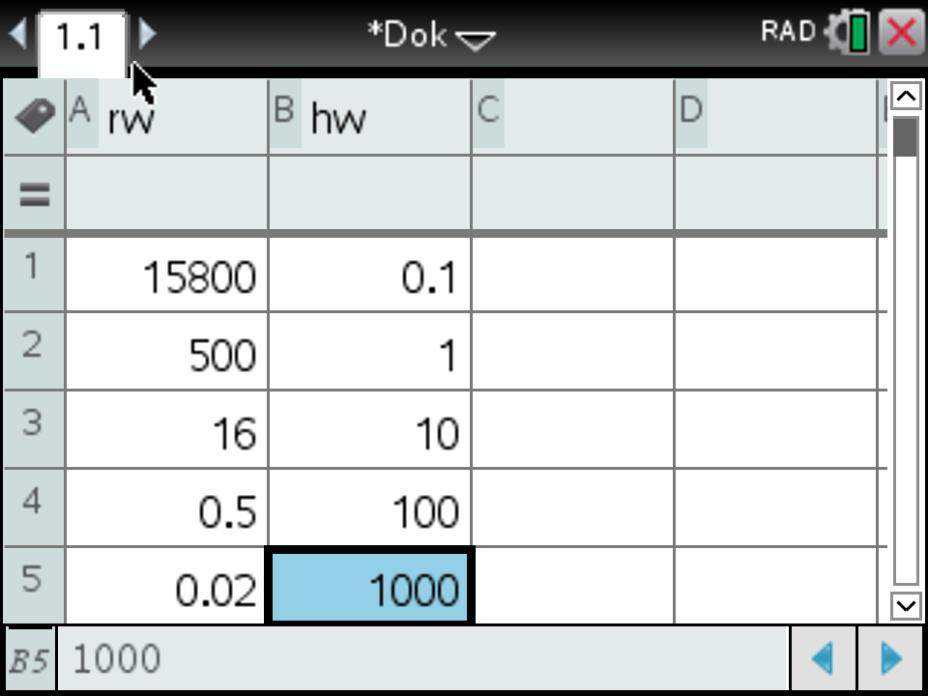
\includegraphics[width=0.8\textwidth]{./pics/RegressionLDR-TI-1.jpg}
	\end{minipage}
	
	
	\begin{minipage}[c][4.5cm][t]{0.48\textwidth}
		\textbf{2.} Füge eine neue Seite \enquote{Data \& Statistics} hinzu (mit \texttt{ctrl} $\rightarrow$ \texttt{+page}). Da wir die Helligkeit in Abhängigkeit vom Widerstand berechnen wollen, kommt der Widerstand auf die Rechtsachse und die Helligkeit auf die Hochachse.
	\end{minipage}
	\hfill
	\begin{minipage}[c][4.5cm][t]{0.48\textwidth}
		\centering
		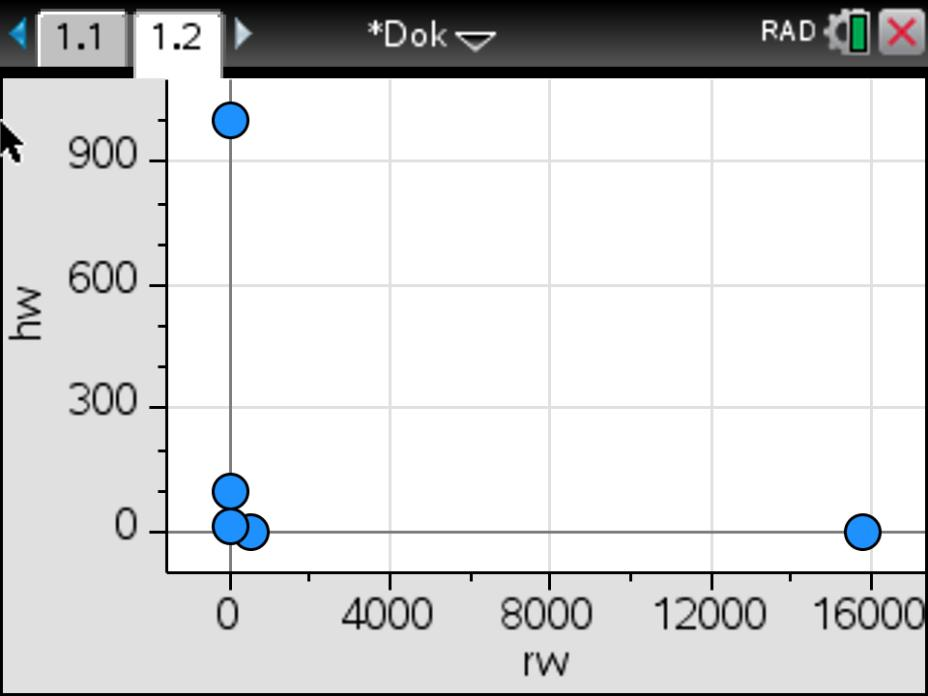
\includegraphics[width=0.8\textwidth]{./pics/RegressionLDR-TI-2.jpg}
	\end{minipage}
	
	\begin{minipage}[c][6cm][t]{0.48\textwidth}
		\textbf{3.} Führe eine Regression durch (\texttt{menu} $\rightarrow$ \texttt{4: Analysieren} $\rightarrow$ \texttt{6: Regression}). Welche Funktionsklasse könnte zu der Verteilung der Werte passen? Falls die ausprobierte Funktionsklasse nicht zu den Werten passt, mache die Regression rückgängig (\texttt{ctrl} $\rightarrow$ \texttt{esc}) und probiere eine andere Funktionsklasse.
		
		\emph{Achtung:} Durch die geringe Auflösung des Taschenrechners können auch passende Funktionen ggf. falsch aussehen.
	\end{minipage}
	\hfill
	\begin{minipage}[c][6cm][t]{0.48\textwidth}
		\centering
		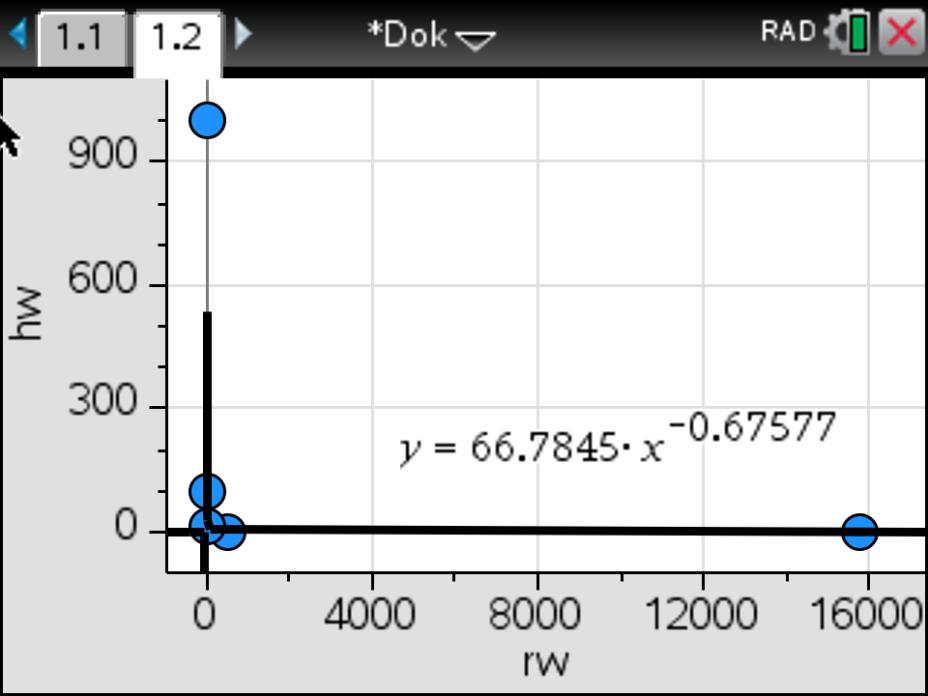
\includegraphics[width=0.8\textwidth]{./pics/RegressionLDR-TI-3.jpg}
	\end{minipage}

	\begin{minipage}[c][3cm][t]{0.48\textwidth}
		\textbf{4.} Übersetze die Funktionsgleichung in den physikalischen Zusammenhang. Für den Widerstand ist das Formelzeichen $R$ festgelegt. Für die Helligkeit wählen wir an dieser Stelle $H$.
	\end{minipage}
	\hfill
	\begin{minipage}[c][3cm][t]{0.48\textwidth}
		\centering
		\vspace{-\baselineskip}
		\begin{align*}
			y &= 66,78 \cdot x^{-0,66} \\
			\downarrow & \hspace{1.6cm}\downarrow \\
			H &= 66,78 \cdot R^{-0,66} \\
			R &\text{ in } \SI{}{\kilo\ohm}, ~ H \text{ in Lux} 
		\end{align*}
	\end{minipage}
\end{zsfg}
\vfill

\begin{zsfg}{Regression mit Geogebra Classic}
	
	\smallskip
	\begin{minipage}[c][4cm][t]{0.48\textwidth}
		\textbf{1.} Starte Geogebra Classic und wähle als Perspektive die Tabellenkalkulation. Übertrage die Daten in die Tabellenkalkulation.
	\end{minipage}
	\hfill
	\begin{minipage}[c][4cm][t]{0.48\textwidth}
		\centering
		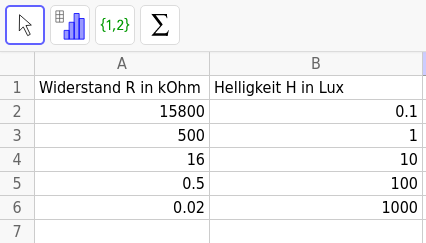
\includegraphics[width=0.8\textwidth]{./pics/RegressionLDR-GGB-1.png}
	\end{minipage}
	
	
	\begin{minipage}[c][4cm][t]{0.48\textwidth}
		\textbf{2.}  Markiere alle Daten und wähle das Werkzeug \texttt{Analyse zweier Variablen}. Die Daten aus Spalte A werden automatisch als x-Koordinate gewählt, die aus Spalte B als y-Koordinate. Bei Bedarf kann dies mit $X \rightleftarrows Y$ vertauscht werden (oben rechts).
	\end{minipage}
	\hfill
	\begin{minipage}[c][4cm][t]{0.48\textwidth}
		\centering
		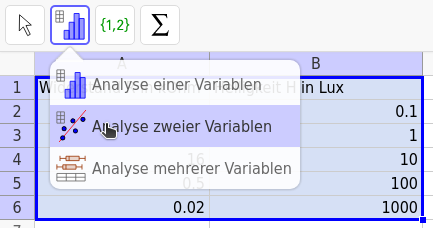
\includegraphics[width=0.8\textwidth]{./pics/RegressionLDR-GGB-2.png}
	\end{minipage}
	
	\begin{minipage}[c][7.5cm][t]{0.48\textwidth}
		\textbf{3.} Führe eine Regression durch, indem du unten links ein passendes Regressionsmodell wählst. Welche Funktionsklasse könnte zu der Verteilung der Werte passen? Falls die ausprobierte Funktionsklasse nicht zu den Werten passt, probiere eine andere Funktionsklasse.
		
		\emph{Hinweis:} Die Anzahl der Nachkommastellen lässt sich in den Einstellungen unter \enquote{Runden} ändern.
	\end{minipage}
	\hfill
	\begin{minipage}[c][7.5cm][t]{0.48\textwidth}
		\centering
		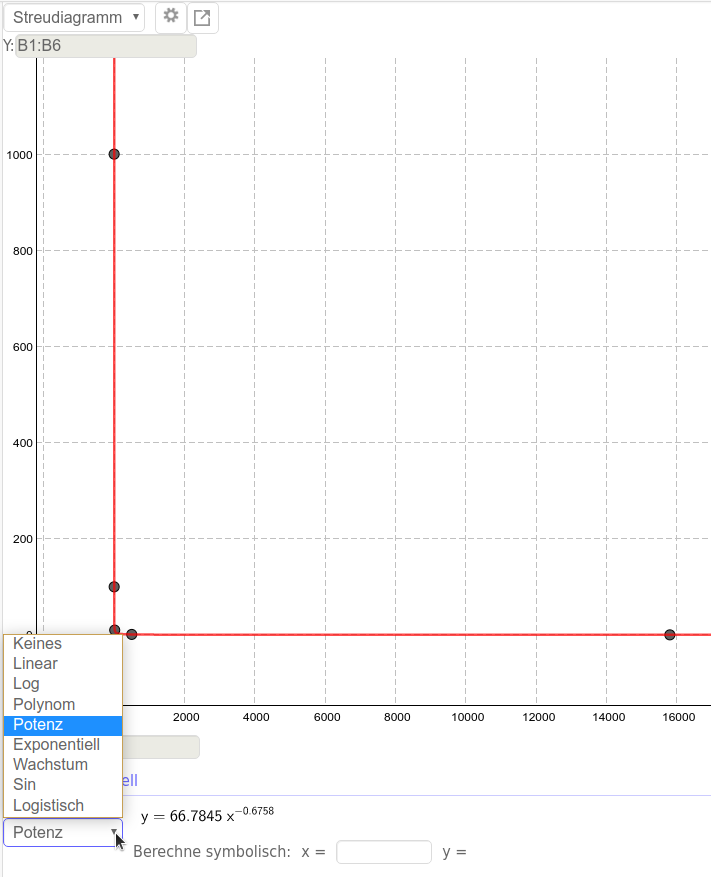
\includegraphics[width=0.8\textwidth]{./pics/RegressionLDR-GGB-3.png}
	\end{minipage}
	
	\begin{minipage}[c][3cm][t]{0.48\textwidth}
		\textbf{4.} Übersetze die Funktionsgleichung in den physikalischen Zusammenhang. Für den Widerstand ist das Formelzeichen $R$ festgelegt. Für die Helligkeit wählen wir an dieser Stelle $H$.
	\end{minipage}
	\hfill
	\begin{minipage}[c][3cm][t]{0.48\textwidth}
		\centering
		\vspace{-\baselineskip}
		\begin{align*}
		y &= 66,78 \cdot x^{-0,66} \\
		\downarrow & \hspace{1.6cm}\downarrow \\
		H &= 66,78 \cdot R^{-0,66} \\
		R &\text{ in } \SI{}{\kilo\ohm}, ~ H \text{ in Lux} 
		\end{align*}
	\end{minipage}
\end{zsfg}
\vfill

%Exkurs/Hintergrund: Wieso ändert sich der Widerstand des LDR, wenn Licht auf ihn trifft? -> Erklärung im Energiebändermodell

% Lichttheremin als Projekt?
\newpage
\section{Temperatur messen}\label{sec:ntc}

\begin{wrapfigure}{r}{0.15\textwidth}
	\centering
	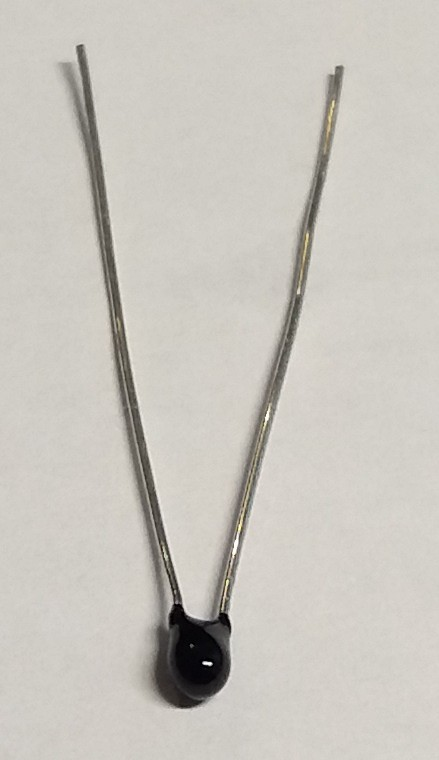
\includegraphics[width=0.1\textwidth]{./pics/ntc.jpg}
	\caption{Ein NTC.}
\end{wrapfigure}
Nicht nur die Helligkeit beeinflusst unseren Alltag, sondern auch die Temperatur. Ganz allgemein ist die Temperatur eine wichtige Größe, die bei vielen Anwendungen eine Rolle spielt und daher erfasst und automatisiert in die Anwendung einfließen sollte: Thermostate regeln die Temperatur im Raum, Wetterstationen geben die Temperatur an und 3D-Drucker regeln die Temperatur der Düse auf eine festgelegte Temperatur, damit der Kunststoff flüssig wird, aber immer noch zäh genug bleibt, um die Figur zu bilden. Häufig wird dabei ein Heißleiter (kurz: NTC, von engl. \emph{negative temperature coefficient}) verwendet - ein elektrischer Widerstand, der auf die Temperatur reagiert.

\begin{ziel}
	\textbf{Frage:} Wie verwendet man einen NTC am Arduino?
\end{ziel}

\begin{aufgabe} \emph{Erste Experimente mit dem NTC}
	\begin{enumerate}[label=\alph*), itemsep=0ex,parsep=0ex]
		\item Baue mithilfe eines Festwiderstands $R_F=\SI{10}{\kilo\ohm}$ und dem NTC einen Spannungsteiler und lies die Spannung am NTC in A0 aus (genau wie beim LDR).
		
		Erwärme den NTC, indem du ihn zwischen Daumen und Zeigerfinger hälst. Beschreibe, wie sich die Spannung am NTC ändert, wenn dieser wärmer wird.
		\item Begründe, dass auch hier gilt:
		\begin{equation*}
			\frac{R_{NTC}}{R_{F}} = \frac{U_{NTC}}{U_{F}}.
		\end{equation*}
		
		Begründe anhand der Formel, wie sich der Widerstand am NTC ändert, wenn dieser wärmer wird.
	\end{enumerate}
\end{aufgabe}

\marginpar{%
	\footnotesize%
	\werkzeug Neues \\
	Werkzeug:\\
	\hyperref[sec:templuft]{Temperatur- und Luft- \\feuchtigkeits-\\sensor}%
}
\begin{projekt}[Digitales Thermometer]\label{proj:thermometer}
	\begin{minipage}{0.58\textwidth}
		Baue ein digitales Thermometer, das die Lufttemperatur im Raum auf dem seriellen Monitor anzeigt!
		
		\bigskip
		Führe dazu mithilfe des rechts abgebildeten Ausschnitts \href{https://pdf1.alldatasheet.com/datasheet-pdf/view/509832/EPCOS/G1541.html}{aus einem Datenblatt} eine Regression durch.
		
		\bigskip
		\textit{\small Das verlinkte Datenblatt ist evtl. nicht das korrekte Datenblatt zu dem NTC. Da die Bauteilnummer bei dem verwendeten Starter Kit nicht angegeben wird, ist eine Zuordnung leider nicht mehr möglich.}

		\vspace{\baselineskip}
	\end{minipage}
	\hfill
	\begin{minipage}{0.38\textwidth}
		\begin{tcolorbox}[sharp corners]
			R/T No. \textbf{7003}
			
			Widerstand bei $\ang{25}$: 
			
			$R_{25}=\SI{10}{\kilo\ohm}$.\\			
			
			\begin{tabular}{l | l | l}
				T (C) & $R_T/R_{25}$ & (\%/K) \\ \hline
				5.0 & 2.3311 & 4.5 \\ \hline
				10.0 & 1.8684 & 4.4  \\ \hline
				15.0 & 1.5075 &  4.2 \\ \hline
				20.0 & 1.224 & 4.1 \\ \hline
				25.0 & 1.0000 & 4.0 \\ \hline
				30.0 & 0.82176 & 3.9 \\ \hline
			\end{tabular}
		\end{tcolorbox}
	\end{minipage}
\end{projekt}

\begin{zsfg}{Heißleiter}
	\begin{minipage}{0.7\textwidth}
		Ein \textbf{Heißleiter}, kurz: \textbf{NTC} (\emph{engl. \textbf{n}egative \textbf{t}emperature \textbf{c}oefficient}), ist ein temperaturabhängiger Widerstand. Wenn es wärmer wird, wird der elektrische Widerstand des NTC kleiner; wenn es kälter wird, wird der elektrische Widerstand des NTC größer.
	\end{minipage}
	\hfill
	\begin{minipage}{0.28\textwidth}
		\begin{minipage}{0.48\textwidth}
			\centering
			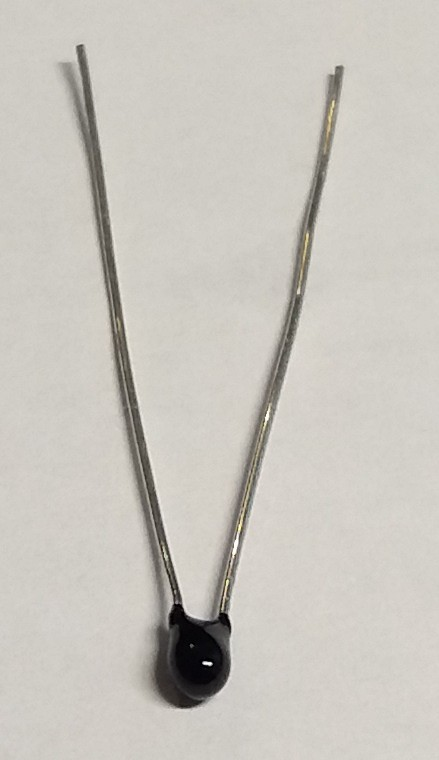
\includegraphics[width=0.9\textwidth, height=2cm]{./pics/ntc.jpg}
		\end{minipage}
		\hfill
		\begin{minipage}{0.48\textwidth}
			\centering
			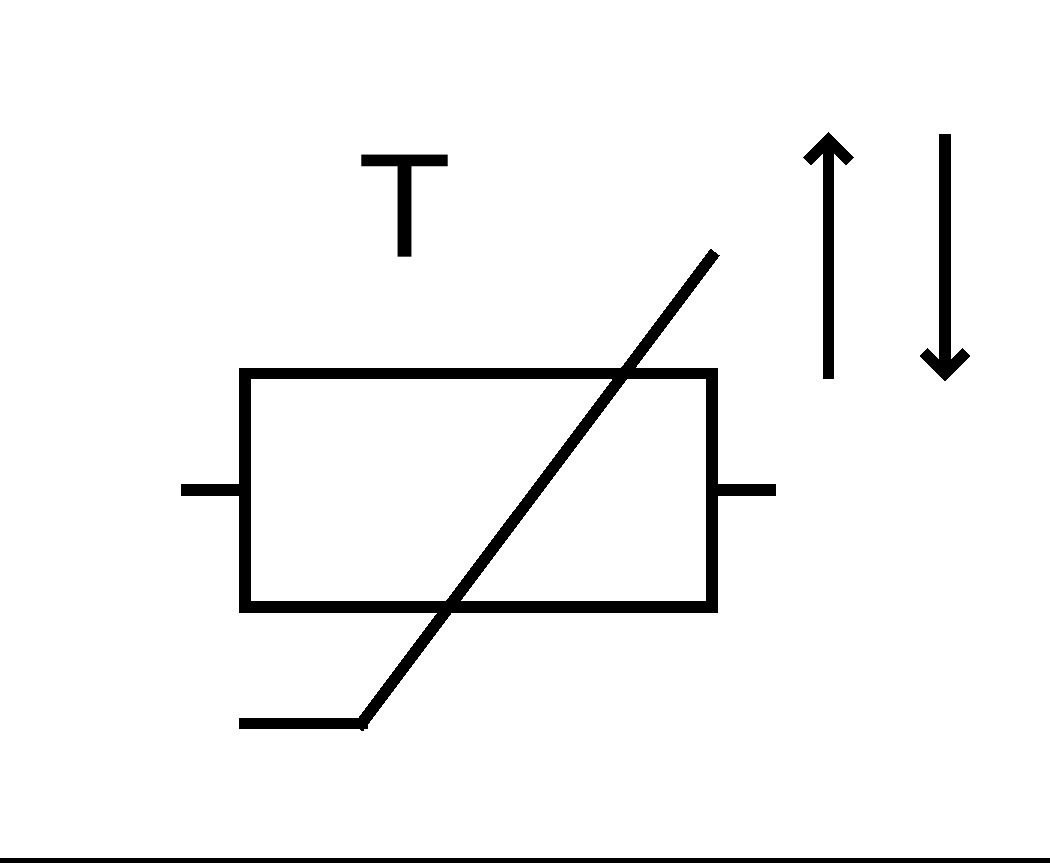
\includegraphics[width=\textwidth]{./pics/ntc-schaltsymbol.png}
		\end{minipage}
	\end{minipage}
	
	\bigskip
	\emph{Anmerkung:}
	
	Es gibt auch Kaltleiter, kurz: \textbf{PTC} (\emph{engl. \textbf{p}ositive \textbf{t}emperature \textbf{c}oefficient}), die ihren Widerstand verringern, wenn es kälter wird, und erhöhen, wenn es wärmer wird. Zusammen genommen bezeichnet man NTC's und PTC's auch als Thermistoren, also als temperaturabhängige Widerstände (engl. \textbf{therm}ally sensitive res\textbf{istor}).
\end{zsfg}

\newpage
\section{Exkurs: Schaltungen mit Transistoren vereinfachen}\label{sec:transistor}

Insbesondere die \enquote{Straßenlampe} benötigt nur ein sehr simples Programm in der Form WENN - DANN - SONST. Für solche Fälle ist der Arduino eigentlich eine überdimensionierte Lösung - viel einfacher, jedenfalls in Bezug auf die Anzahl der Bauteile, ist die Umsetzung dieser Schaltung mithilfe eines Transistors. Dieser ist (unter anderem) ein elektronischer Schalter, mit dem sich das WENN - DANN - SONST - Verhalten ganz ohne Programm umsetzen lässt.

\begin{ziel}
	\textbf{Frage:} Wie verwendet man einen Transistor?
\end{ziel}

\medskip
\begin{minipage}{0.85\textwidth}
	Ein Transistor hat drei Anschlüsse, die als Kollektor (\textbf{C} von engl. \emph{collector}), Basis (\textbf{B}) und Emitter (\textbf{E}) bezeichnet werden. Wenn man auf die abgeflachte Seite des Transistors schaut, sind die drei Pins in der genannten Reihenfolge angeordnet. Im Folgenden geht es zunächst um deren Grundfunktionen.
\end{minipage}
\hfill
\begin{minipage}{0.13\textwidth}
	\centering
	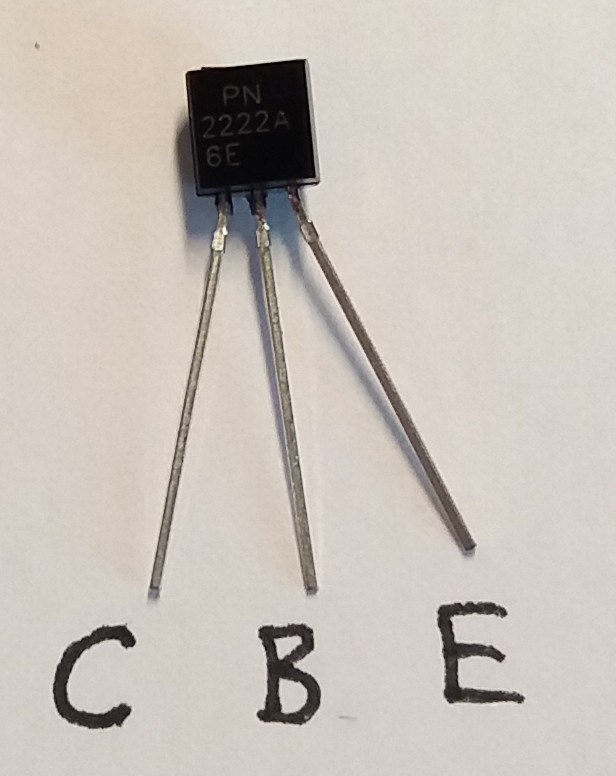
\includegraphics[width=0.77\textwidth]{./pics/transistor.jpg}
\end{minipage}

\medskip

\begin{aufgabe} \emph{Digitalpins verstehen}
	
	Befolge die unten angegebenen Schritte und stelle Schlussfolgerungen über die Funktionsweise eines Transistors an.
	\begin{enumerate}[label=\alph*), itemsep=0mm,parsep=0mm]
		\item Baue die unten abgebildeten Schaltungen nacheinander auf. Spiele für die zweite Schaltung ein einfaches Blink-Programm auf den Arduino.
		\begin{figure}[H]
			\centering
			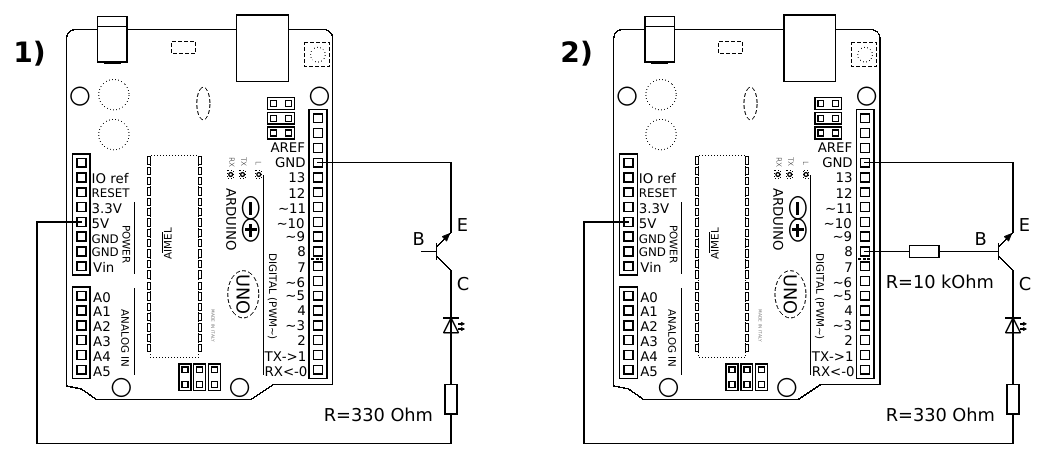
\includegraphics[width=0.75\textwidth]{./Zeichnungen/Schaltplan-Transistor-verstehen.png}
		\end{figure}
		\item Ersetze den $\SI{10}{\kilo\ohm}$ Widerstand durch einen $\SI{100}{\kilo\ohm}$ Widerstand.
	\end{enumerate}
\end{aufgabe}

\marginpar{%
	\footnotesize%
	\werkzeug Neues \\
	Werkzeug:\\
	\hyperref[kap:e-motor]{Elektromotor}%
}
\begin{aufgabe} \emph{Vermessung}
	
	\medskip
	\begin{minipage}{0.58\textwidth}
		Um den Transistor zielgerichtet nutzen zu können, muss man die Spannung $U_{BE}$ zwischen Basis und Emitter kennen, bei der der Transistor anfängt, durchzuschalten. Dazu dient die rechts abgebildete Schaltung.
		
		Das Potentiometer lässt sich wieder in zwei Teilwiderstände $R_1$ und $R_2$ zerlegen, an denen die Spannung $U_1$ bzw. $U_2$ abfällt. Erkläre, wie der Widerstand $R_2$ und die Spannung $U_{BE}$ zusammenhängen.
	\end{minipage}
	\hfill
	\begin{minipage}{0.38\textwidth}
		\centering
		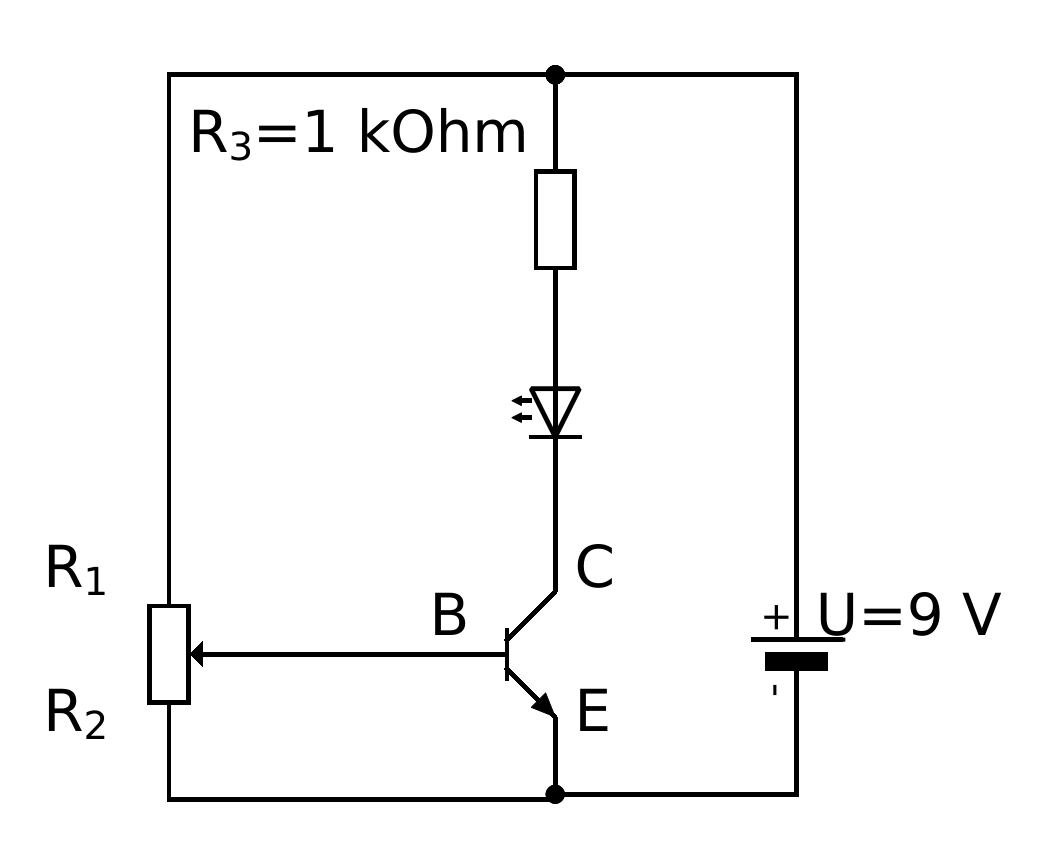
\includegraphics[width=\textwidth]{./Zeichnungen/Schaltplan-U-BE-Messung1.png}
	\end{minipage}

	\begin{minipage}[c][8cm][t]{0.58\textwidth}
		Baue die Schaltung nun auf. Um die Spannung $U_{BE}$ messen zu können, wird ein Arduino ergänzt, der die Spannung in A0 ausliest und auf dem seriellen Monitor ausgibt. 
		
		Bestimme so die Grenzspannung $U_{BE}$, ab der der Transistor anfängt zu schalten, sodass die LED leuchtet.
		
		\begin{center}
			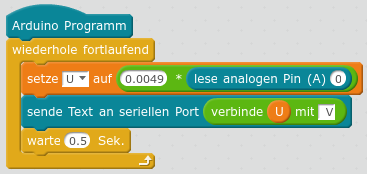
\includegraphics[width=0.8\textwidth]{./pics/Programm-Spannung-messen.png}
		\end{center}
	\end{minipage}
	\hfill
	\begin{minipage}[c][8cm][t]{0.38\textwidth}
		\centering
		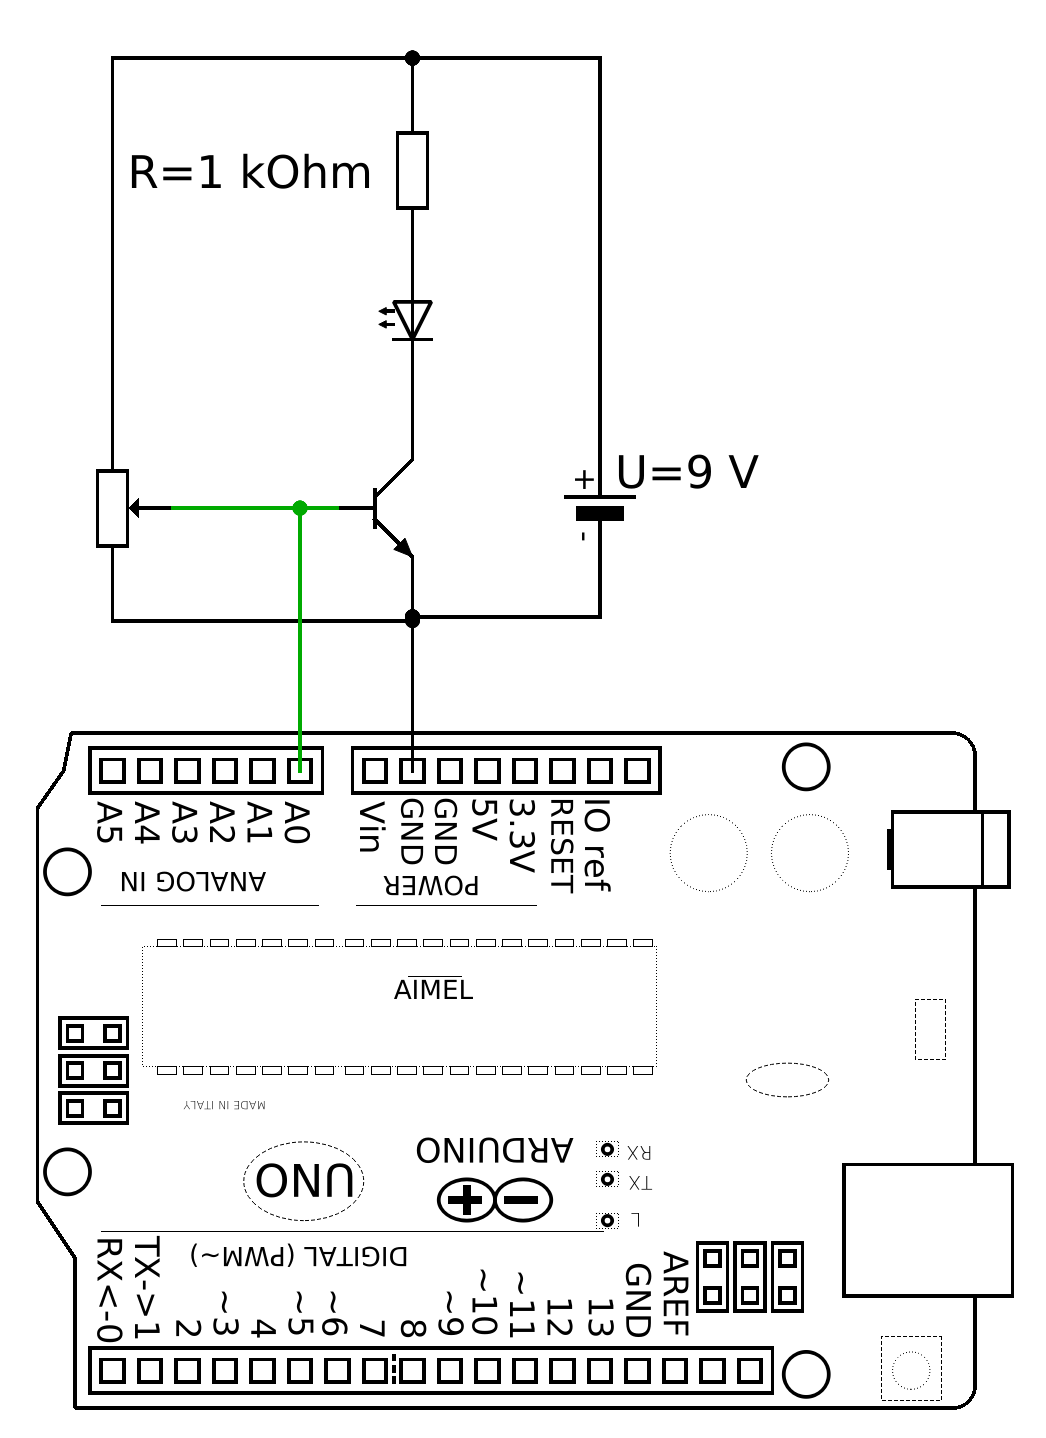
\includegraphics[width=\textwidth]{./Zeichnungen/Schaltplan-U-BE-Messung.png}
	\end{minipage}
\end{aufgabe}

\begin{projekt}[Straßenlampe ohne Mikrocontroller\label{proj:strassenlampeomc}]
	\begin{minipage}{0.58\textwidth}
		Nun kann die Straßenlampe auch ohne Arduino realisiert werden. Dazu wird statt des Potentiometers ein Spannungsteiler mit einem LDR und einem Festwiderstand aufgebaut (siehe Schaltplan rechts).
		
		Bestimme die Größe des Festwiderstands $R_F$ so, dass der Transistor schaltet, wenn die Größe des LDR $R_{LDR}=\SI{7}{\kilo\ohm}$ beträgt.
		
		\emph{Tipps:}
		\begin{itemize}[itemsep=0mm, parsep=0mm]
			\item Nutze die Spannungsteilerformel.
			\item Nutze $U_{LDR}=U_{BE}$. Ab welcher Spannung schaltet der Transistor?
		\end{itemize}
	\end{minipage}
	\hfill
	\begin{minipage}{0.4\textwidth}
		\centering
		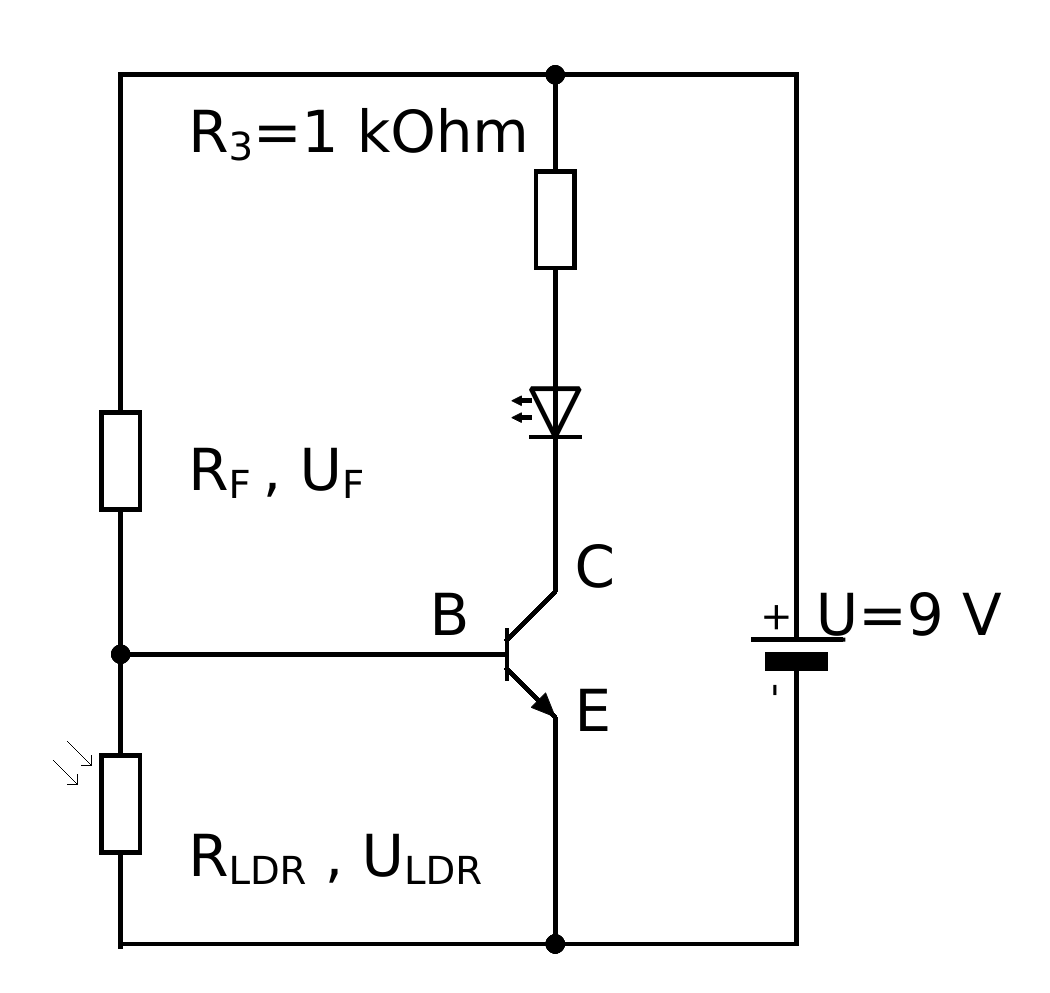
\includegraphics[width=\textwidth]{./Zeichnungen/Schaltplan-Strassenlampe-ohne-mC.png}
	\end{minipage}
	
	\bigskip
	Baue die Schaltung danach auf und teste sie.
\end{projekt}

\begin{zsfg}{Der Transistor}
	
	\medskip
	\begin{minipage}{0.7\textwidth}
		Ein Transistor hat drei Anschlüsse, die als Kollektor (\textbf{C} von engl. \emph{collector}), Basis (\textbf{B}) und Emitter (\textbf{E}) bezeichnet werden. Wenn man auf die abgeflachte Seite des Transistors schaut, sind die drei Pins in der genannten Reihenfolge angeordnet.
	\end{minipage}
	\hfill
	\begin{minipage}{0.28\textwidth}
		\begin{minipage}{0.48\textwidth}
			\centering
			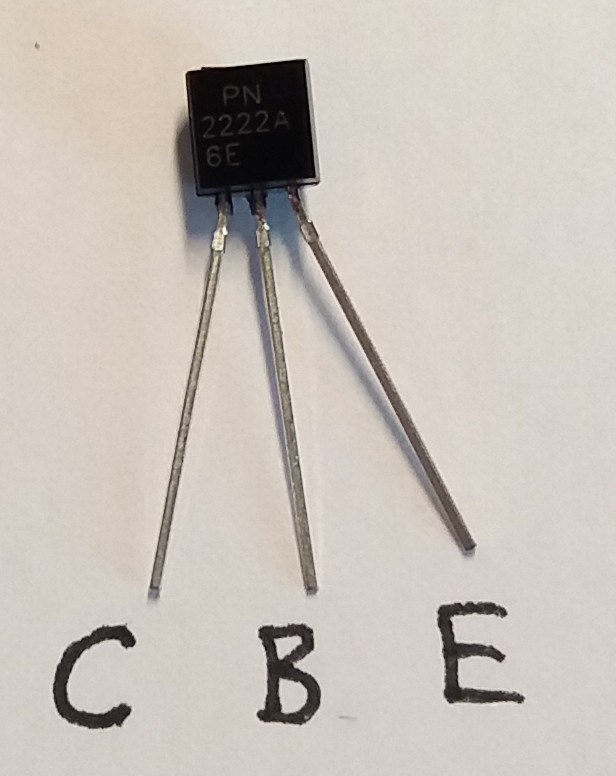
\includegraphics[width=0.9\textwidth, height=2cm]{./pics/transistor.jpg}
		\end{minipage}
		\hfill
		\begin{minipage}{0.48\textwidth}
			\centering
			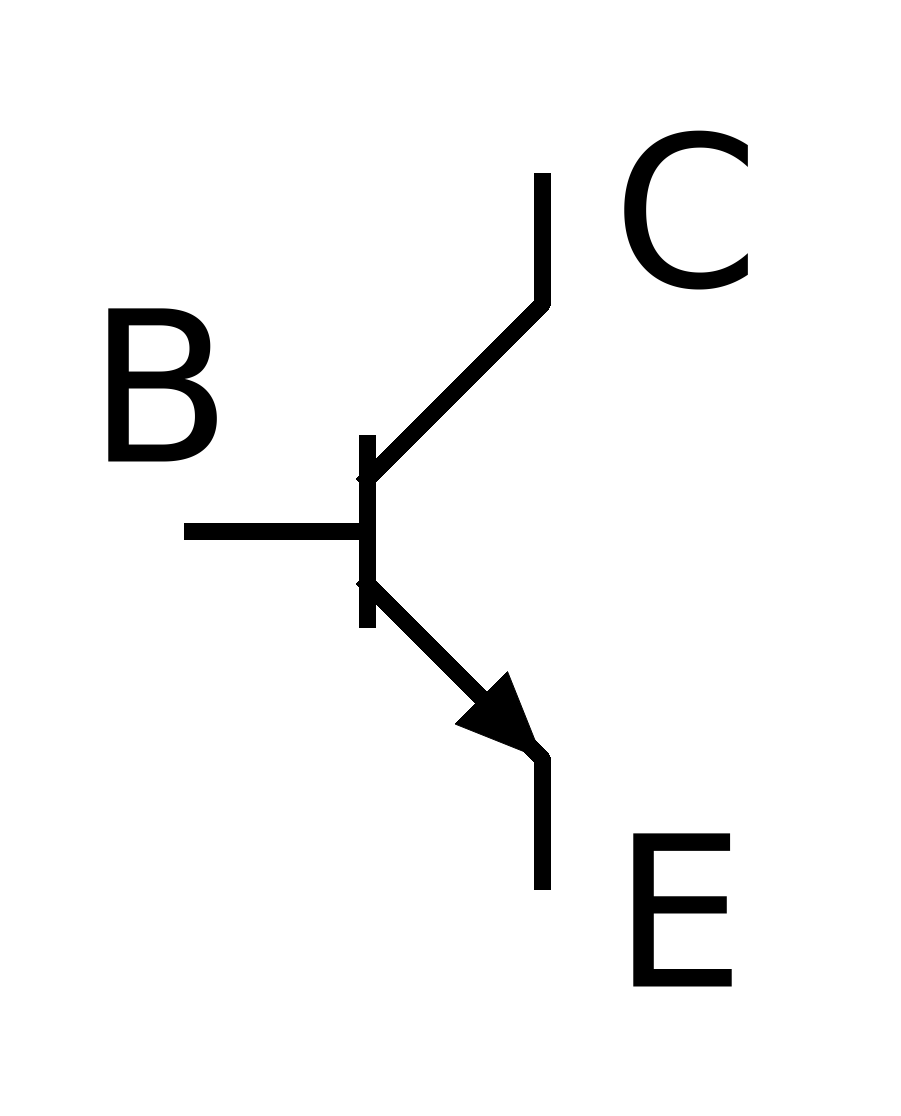
\includegraphics[width=0.9\textwidth, height=2cm]{./pics/transistor-schaltsymbol.png}
		\end{minipage}
	\end{minipage}
	
	\medskip
	Transistoren dienen als elektronische Schalter oder Verstärker (letzteres wird im Kapitel \ref{kap:e-motor} zu Motoren genutzt). Als Schalter lassen sie sich nutzen, weil die Strecke vom Kollektor zum Emitter ohne Weiteres nicht leitet. Erst wenn zwischen Basis und Emitter eine Spannung $U_{BE} \approx \SI{0,6}{\volt}$ anliegt, fließt \emph{zwischen Basis und Emitter ein schwacher Strom}, der den Transistor mit Elektronen flutet und es dadurch ermöglicht, dass \emph{zwischen Kollektor und Emitter ein starker Strom} fließen kann.
	
	Die Möglichkeit, mit Transistoren automatisierte Schalter herzustellen und dadurch Programme physikalisch abzubilden, macht Transistoren zur Grundlage von Mikrocontrollern und Computern und damit zu einer der wichtigsten Erfindungen des 20. Jahrhunderts. Schon auf dem kleinen integrierten Schaltkreis des Arduino, dem ATMEGA328P, sind Millionen von Transistoren verbaut. Wenn ein Digitalpin des Arduino auf HIGH gestellt wird, dann wird intern ein Transistor geschaltet.
	
	Es gibt verschiedene Bauarten für Transistoren. Im hier verwendeten Starter Kit sind zwei npn-Transistoren (Pn2222) vorhanden, was bedeutet, dass darin zwei n-dotierte und eine p-dotierte Schicht in der Mitte verbaut sind. npn-Transistoren müssen mit einer n-Schicht (normalerweise der Emitter) mit GND verbunden sein.
\end{zsfg}


\section{Das EVA-Prinzip}

Allmählich hat sich eine Vielzahl an elektrischen Bauteilen angesammelt, die in diesem Skript genutzt wurden. Um nicht den Überblick zu verlieren, wären Kategorien praktisch, mit denen man Bauteile und technische Systeme im Allgemeinen einordnen kann.

\begin{ziel}
	\textbf{Frage:} Wie lassen sich elektrische Bauteile und technische Systeme kategorisieren?
\end{ziel}
\marginpar{%
	\textattachfile[description={Folie zu Kap. \thechapter, Bauteilkategorisierung}]{./Auftraege/kap5-bauteilkategorisierung.pdf}{%
		\footnotesize\folie Folie%
	}%
	\footnotesize%
	%\folie \href{run:./Auftraege/kap5-bauteilkategorisierung.pdf}{Folie} \\
	\\öffnen%
}

\begin{aufgabe}
	Du hast bisher (mindestens) folgende Bauteile verwendet:
	
	\medskip
	\begin{center}
		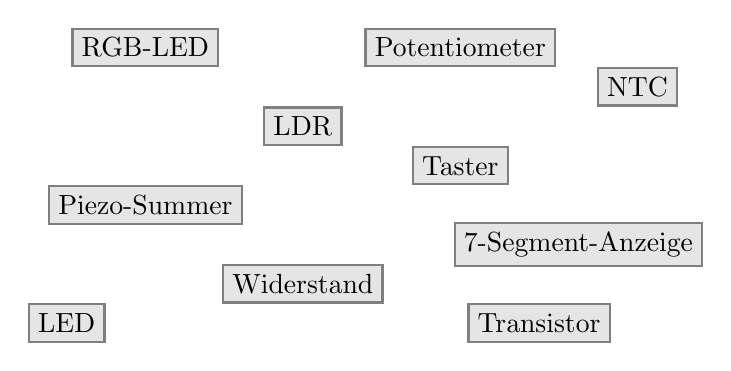
\begin{tikzpicture}[rect/.style={shape=rectangle, thick, draw=black!50, fill=black!10}]
		\node at (0,0) [rect] {LED};
		\node at (3,0.5) [rect] {Widerstand};
		\node at (1,3.5) [rect] {RGB-LED};
		\node at (6.5,1) [rect] {7-Segment-Anzeige};
		\node at (5,2) [rect] {Taster};	
		\node at (1,1.5) [rect] {Piezo-Summer};
		\node at (5,3.5) [rect] {Potentiometer};
		\node at (3,2.5) [rect] {LDR};
		\node at (7.25,3) [rect] {NTC};
		\node at (6,0) [rect] {Transistor};
		\end{tikzpicture}
	\end{center}
	
	\medskip
	Ordne sie nach ihrer Funktion in vier Gruppen.
\end{aufgabe}

\begin{zsfg}{Bauteilkategorien}
	Elektrische Bauteile lassen sich grob in vier Gruppen einordnen:
	
	\begin{itemize}[itemsep=0ex]
		\item \textbf{Aktive Bauteile} übernehmen in der Schaltung eine steuernde Funktion; sie können elektrische Signale umwandeln oder modifizieren. Unter den aktiven Bauteilen haben zwei Gruppen eine besondere Bedeutung:
		\begin{itemize}[itemsep=0mm,parsep=0mm]
			\item \textbf{Sensoren} (auch Fühler genannt) sind elektrische Bauteile, die eine physikalische Größe aus der Umwelt (Temperatur, Helligkeit, Luftdruck oder auch ein mechanischer Druck mit dem Finger) in eine elektrische Größe (Widerstand, Spannung, elektrisches Potential, Stromstärke) umwandeln. Dadurch werden die physikalischen Größen aus der Umwelt einer elektronischen Verarbeitung zugänglich.
			\item \textbf{Aktoren} (auch Aktuatoren genannt) sind elektrische Bauteile, die eine elektrische Größe in eine mechanische (Bewegung, Schallwellen) oder andere Größe (Temperatur, Licht, \dots) umwandeln. Sie ermöglichen, dass die elektronische Verarbeitung zu Handlungen bzw. Konsequenzen führen kann.
		\end{itemize}
		\item \textbf{Passive Bauteile} haben eine feste Größe, die sich nicht ändert (z.\,B. ein ohmscher Widerstand). Sie sind nicht nur unabhängig von physikalischen Größen in der Umgebung, sondern auch von den elektrischen Größen (z.\,B. ein ohmscher Widerstand hat unabhängig von der anliegenden Spannung den gleichen Wert). 
	\end{itemize}
\end{zsfg}

Abgesehen von der bisweilen nicht ganz eindeutigen Zuordnung zu einer Bauteilgruppe wird hier ein allgemeines Prinzip deutlich, das sich eignet, um technische, aber auch biologische Systeme zu beschreiben.

\begin{zsfg}{Das EVA-Prinzip}
	
	Technische Systeme lassen sich nach ihrer Funktion in drei Einheiten zerlegen: Eingabeeinheit, Verarbeitungseinheit, Ausgabeeinheit.
	
	\bigskip
	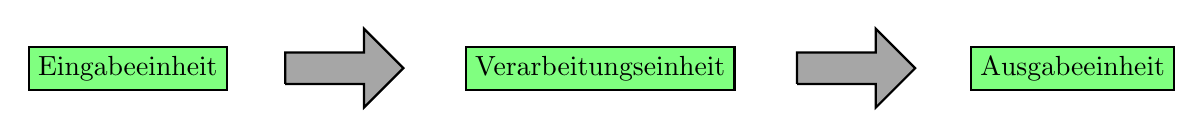
\begin{tikzpicture}[rect/.style={shape=rectangle, thick, draw=black, fill=green!50}]
	\node at (0,0) [rect] {Eingabeeinheit};
	\draw [fill=gray!70, thick] (2,-0.2) -- ++(1,0)-- ++(0,-0.3) -- ++(0.5,0.5) -- ++(-0.5,0.5) -- ++(0,-0.3) -- ++(-1,0) -- ++(0,-0.4);
	\node at (6,0) [rect] {Verarbeitungseinheit};
	\draw [fill=gray!70, thick] (8.5,-0.2) -- ++(1,0)-- ++(0,-0.3) -- ++(0.5,0.5) -- ++(-0.5,0.5) -- ++(0,-0.3) -- ++(-1,0) -- ++(0,-0.4);
	\node at (12,0) [rect] {Ausgabeeinheit};
	\end{tikzpicture}
	
	\bigskip
	Mit dem EVA-Prinzip wird die grundlegende Reihenfolge der Verarbeitung von Daten charakterisiert. Die Einheiten bestehen dabei nicht nur aus den Bauteilen, sondern beinhalten auch die Art der Verarbeitung, also zum Beispiel das Programm auf dem Arduino. Insbesondere sind die Einheiten nicht gleichbedeutend mit den oben genannten Bauteilgruppen!
\end{zsfg}

\smallskip
\emph{\bfseries Beispiel Dämmerungsschaltung:}

Der Spannungsteiler von Festwiderstand und LDR ermöglicht die Eingabe von Daten zur Helligkeit, also kann dies als Eingabeeinheit angesehen werden. Auf dem Arduino werden die elektrischen Signale entsprechend des laufenden Programms verarbeitet; dies ist die Verarbeitungseinheit. Letztlich erfolgt die Ausgabe durch das Leuchten einer LED, wenn es dunkel ist, bzw. durch das Nicht-Leuchten der LED. Die LED mit zugehörigem Vorwiderstand kann als Ausgabeeinheit angesehen werden.

\smallskip
\emph{\bfseries Beispiel Mensch:}

Unsere Sinne (Augen zum Sehen, Ohren zum Hören, \dots) bilden die Eingabeeinheiten des Systems Mensch. Im Gehirn und den weiteren Nervenbahnen im Körper werden die Signale verarbeitet. Dies ist die Verarbeitungseinheit des Menschen. Schließlich kommt es zum Beispiel zu einer Bewegung (Musik leiser drehen, Augen zukneifen, sprechen mit dem Mund \dots) - dies gehört zu den Ausgabeeinheiten des Menschen.

\begin{aufgabe} \emph{Kleines Begriffstraining}
	
	\begin{enumerate}[label=\alph*),itemsep=0ex,parsep=0ex]
		\item Kategorisiere die \emph{Dimmbare Lampe} (s. S. \pageref{proj:dimmlampe}) nach dem EVA-Prinzip.
		\item Kategorisiere das \emph{Digitalthermometer} (s. S. \pageref{proj:thermometer}) nach dem EVA-Prinzip.
	\end{enumerate}
\end{aufgabe}
\marginpar{%
	\footnotesize%
	\werkzeug Neues \\
	Werkzeug:\\
	\hyperref[sec:infrarot-fern]{Infrarot-Fernbedienung}%
}


\newpage
\section{Vermischte Übungen}

\begin{aufgabe} \emph{Pulsweitenmodulation}
	
	\begin{enumerate}[label=\alph*), itemsep=0mm,parsep=0mm]
		\item Berechne die mittlere Spannung, die mit dem Befehl \button{setze PWM-Pin 5 Ausgang auf 138} ausgegeben wird.
		\item Mit dem in a) genannten Befehl wird eine Pulsweitenmodulation durchgeführt. Erkläre, was darunter zu verstehen ist.
		\item Jannik meint: \enquote{Mit dem Befehl in a) kann ich eine blaue LED auch ohne Vorwiderstand betreiben, denn die halten die berechnete Spannung aus.} Nimm dazu Stellung.
	\end{enumerate}
	% Fading, mittl. Spannung zu Befehl ausrechnen, erklären, was passiert (-> mittl. Spannung klein genug für blaue LED, aber nicht rote LED; jemand behauptet, dass man blaue LED anschließen darf, aber rote nicht)
	% Hexadezimalcode in Dezimalzahlen / PWM-Werte umrechnen
\end{aufgabe}

\begin{aufgabe} \emph{Hexadezimalzahlen und RGB-Code}
	
	\begin{enumerate}[label=\alph*), itemsep=0mm,parsep=0mm]
		\item Eine Farbe lässt sich im RGB-Farbcode zum Beispiel durch \texttt{\#10FFC7} codieren. Erläutere, wie dieser Code aufgebaut ist.
		\item Berechne die Dezimalzahlen zu dem RGB-Code aus a).
		\item Die Dezimalzahlen lassen sich als PWM-Werte nutzen, wenn man eine RGB-LED am Arduino anschließt. Bestimme anhand des RGB-Hexadezimal-Farbcodes die PWM-Werte für Rot, Grün und Blau in der folgenden Tabelle.
	\end{enumerate}
	\vspace{-\baselineskip}
	\begin{table}[H]
		\centering
		\begin{minipage}[c]{\textwidth}
			\begin{tabu} to \textwidth {X[L,2]X[L]X[L]|X[L,2]X[L]X[L]}
				\toprule
				\textbf{Farbe} & \textbf{Hex-Code} & \textbf{PWM-Werte} & \textbf{Farbe} & \textbf{Hex-Code} & \textbf{PWM-Werte} \\
				\midrule
				\textcolor{navyblue}{\rule{1cm}{0.4cm}} NavyBlue	& \texttt{\# 000080} &  & \textcolor{aquamarine}{\rule{1cm}{0.4cm}} Aquamarine & \texttt{\# 7FFFD4} &  \\ 
				\textcolor{sandybrown}{\rule{1cm}{0.4cm}} SandyBrown	& \texttt{\# F4A460} &  & \textcolor{seagreen}{\rule{1cm}{0.4cm}} SeaGreen & \texttt{\# 2E8B57} &  \\
				\textcolor{coral}{\rule{1cm}{0.4cm}} Coral	& \texttt{\# FF7F50} &  & \textcolor{darkorchid}{\rule{1cm}{0.4cm}} DarkOrchid & \texttt{\# 9932CC} &  \\
				\bottomrule
			\end{tabu}
		\end{minipage}
		\label{tab:rgb-codes2}
	\end{table}
	\emph{Zur Kontrolle:} \href{http://www.farb-tabelle.de/de/rgb2hex.htm}{www.farb-tabelle.de}
\end{aufgabe}

%Lösung zur Tabelle:
% NavyBlue: 0,0,128
% Aquamarine: 127,255,212
% Sandybrown: 244,164,96
% SeaGreen: 46, 139, 87
% Coral: 255,127,80
% DarkOrchid: 153, 50, 204

\begin{aufgabe} \emph{Spannungsmessung}
	
	\begin{wrapfigure}{r}{0.4\textwidth}
		\centering
		\vspace{-2\baselineskip}
		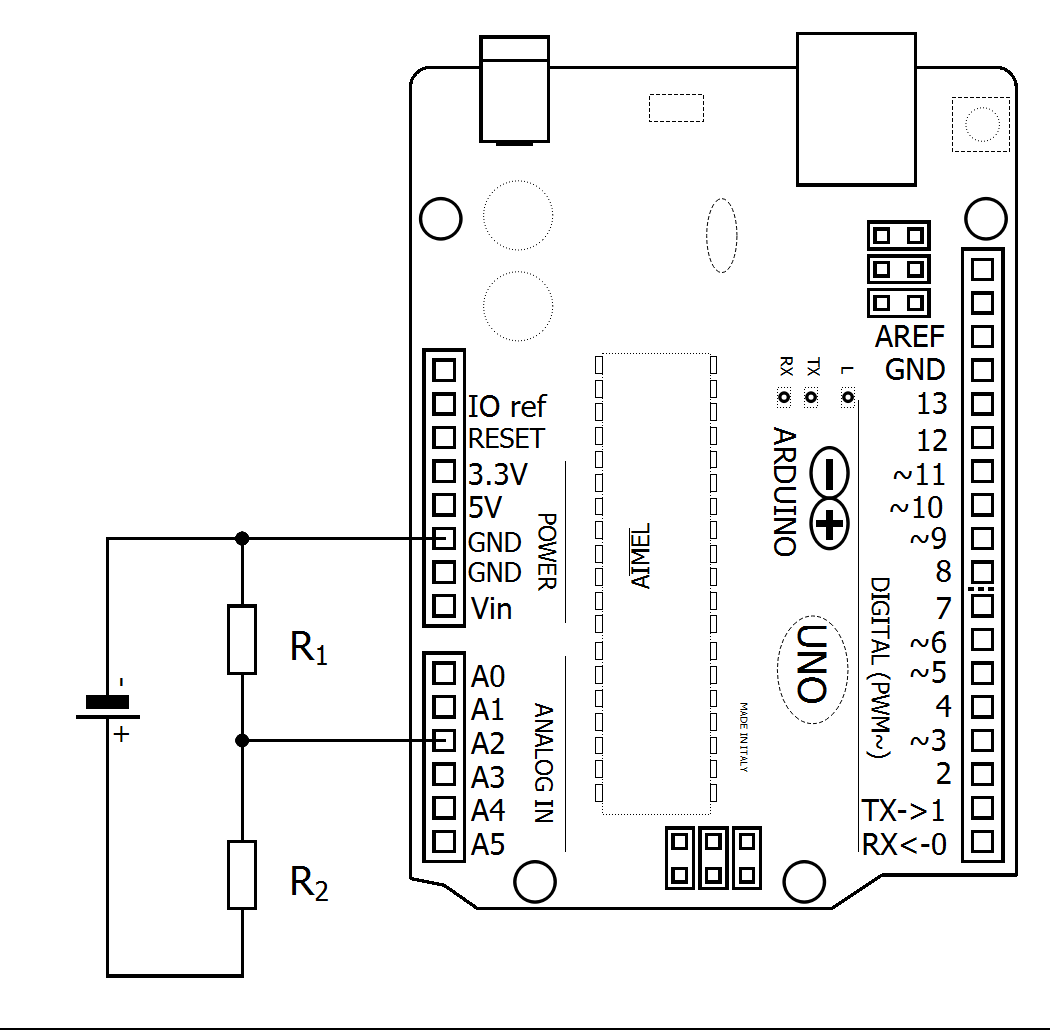
\includegraphics[width=0.4\textwidth]{./Zeichnungen/schaltplan-spannungsmessung.png}
	\end{wrapfigure}
	Mit der rechts abgebildeten Schaltung sollen am Arduino Spannungen an der Batterie bis zu $\SI{15}{\volt}$ gemessen werden.
	\begin{enumerate}[label=\alph*),itemsep=0mm,parsep=0mm]
		\item Nenne mögliche, sinnvolle Größen für die Widerstände $R_1$ und $R_2$.
		\item Im analogen Eingang A2 wird ein Wert von 789 gemessen. Berechne die Spannung an der Batterie.
	\end{enumerate}
\end{aufgabe}

\newpage
\begin{aufgabe} \emph{Potentiometer}
	
	\begin{enumerate}[label=\alph*), itemsep=0mm]
		\item Erläutere die Funktionsweise eines Potentiometers und nenne ein Einsatzbeispiel.
		\item Skizziere, wie man ein Potentiometer am Arduino anschließt.
		\item Ein Potentiometer hat einen Gesamtwiderstand von $R_{ges}=\SI{10}{\kilo\ohm}$. Der mittlere Kontakt wird im analogen Eingang A0 ausgelesen und liefert einen Analogwert von 824. Berechne, wie groß die Teilwiderstände sind. 
	\end{enumerate}
\end{aufgabe}

\begin{aufgabe} \emph{Dimmbarer Lautsprecher}
	
	\begin{wrapfigure}{r}{0.4\textwidth}
		\centering
		\vspace{-1\baselineskip}
		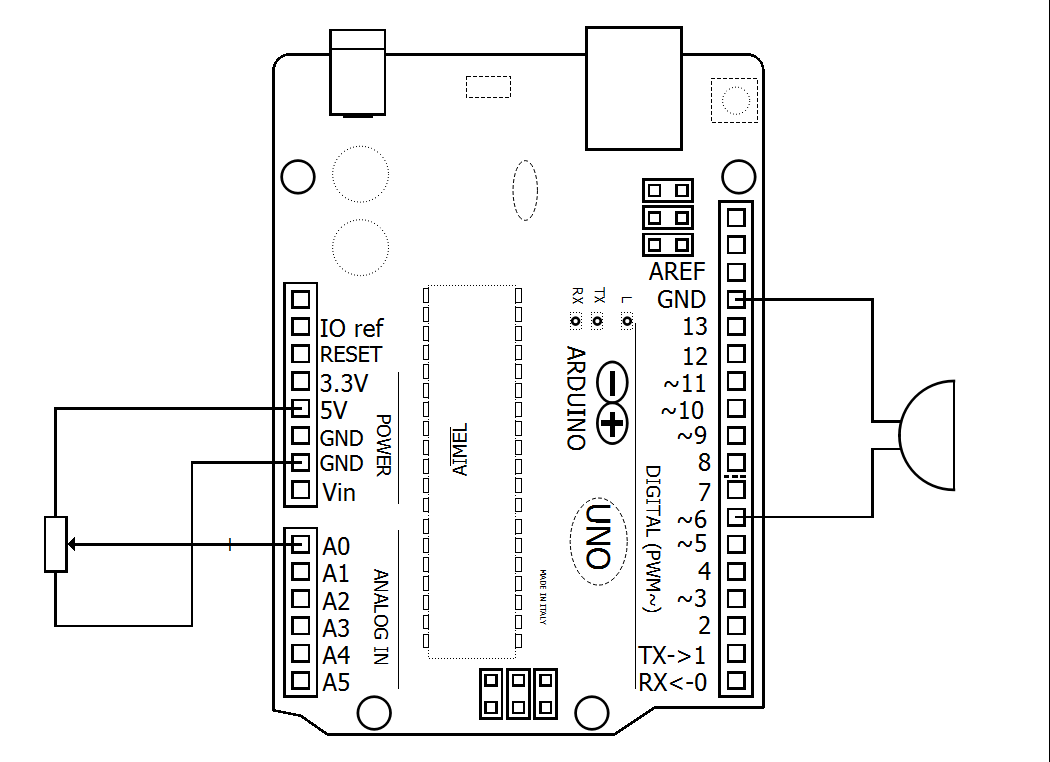
\includegraphics[width=0.4\textwidth]{./Zeichnungen/schaltplan-dimmbarer-lautsprecher.png}
	\end{wrapfigure}
	Der Schaltplan rechts zeigt ein Potentiometer, dessen mittlerer Kontakt am analogen Eingang A0 eines Arduino angeschlossen ist. Auf der anderen Seite ist ein Piezo-Summer an Digitalpin 6 des Arduino angeschlossen.
	
	Entwickle mit den unten abgebildeten Befehlen ein Programm, das dafür sorgt, dass die Lautstärke des Piezo-Summers durch das Potentiometer gedimmt werden kann. Das Programm soll in einem Struktogramm dokumentiert werden.
	
	\begin{figure}[H]
		\centering
		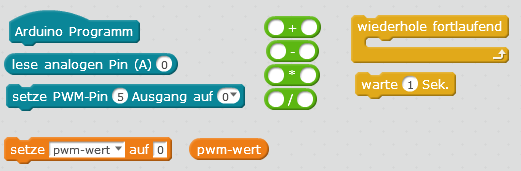
\includegraphics[width=0.8\textwidth]{./pics/befehle-fuer-dimmbaren-lautsprecher.png}
	\end{figure}
\end{aufgabe}

\begin{aufgabe} \emph{LDR und NTC - Basics}
	
	\medskip
	\begin{minipage}{0.59\textwidth}
		\begin{enumerate}[label=\alph*), itemsep=0mm, parsep=0mm]
			\item Nenne jeweils einen Einsatzzweck für einen LDR und einen NTC.
			\item Beschreibe das Widerstandsverhalten eines LDR (eines NTC), wenn sich die Helligkeit (die Temperatur) verringert.
			\item Ein NTC ist in einem Spannungsteiler mit einem Festwiderstand mit $R_F=\SI{10}{\kilo\ohm}$ am Arduino angeschlossen (s. Schaltplan rechts). Im analogen Eingang A0 wird ein Wert von 643 gemessen. Berechne die Größe des Widerstands des NTC.
		\end{enumerate}
	\end{minipage}
	\hfill
	\begin{minipage}{0.39\textwidth}
		\centering
		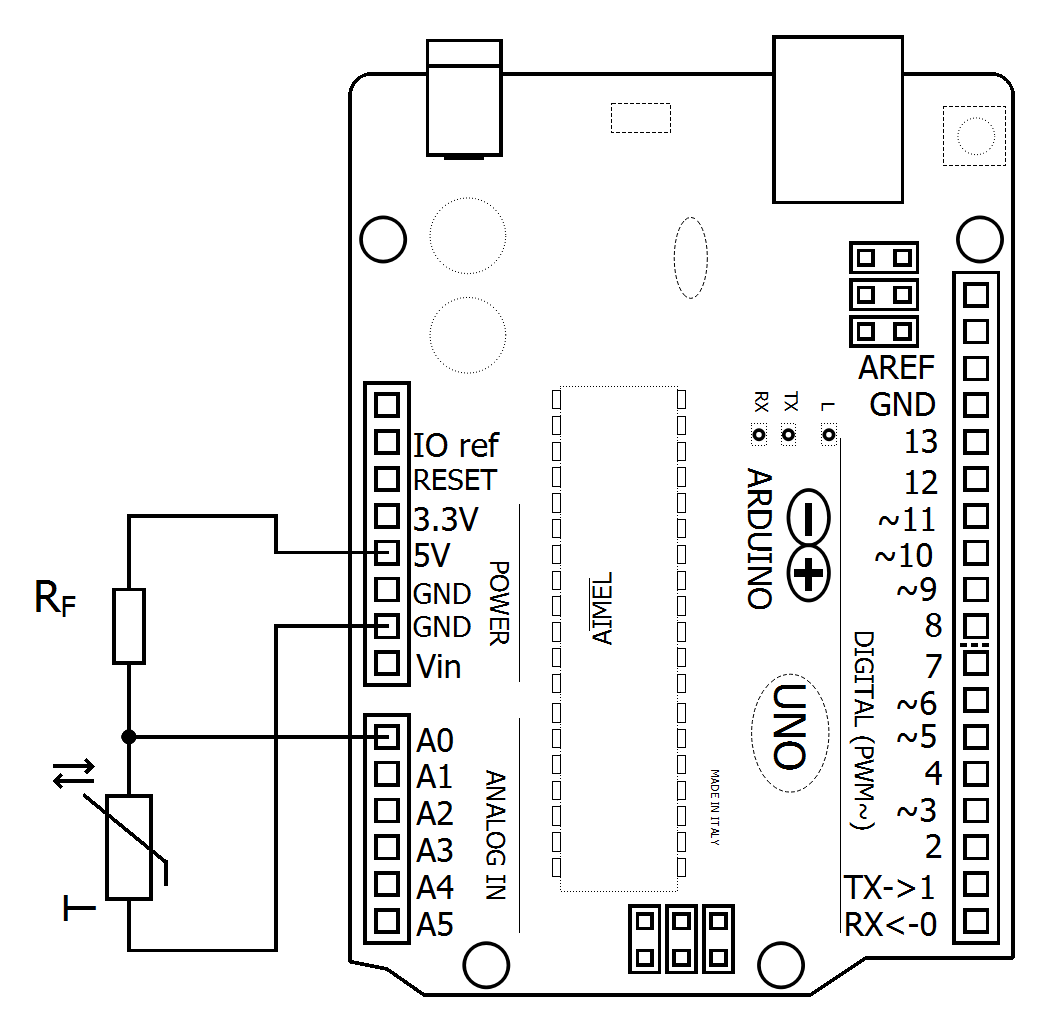
\includegraphics[width=\textwidth]{./Zeichnungen/schaltplan-ntc-an-arduino.png}
	\end{minipage}

	\begin{minipage}{0.48\textwidth}
		\begin{enumerate}[label=\alph*), itemsep=0mm, parsep=0mm]
			\setcounter{enumi}{3}
			\item Die Tabelle unten zeigt für den verwendeten NTC, welche Widerstandswerte $R$ zu welcher Temperatur $T$ gehören. Bestimme mit Hilfe einer quadratischen Regression einen funktionalen Zusammenhang zwischen $R$ und $T$ und berechne damit die Temperatur, die zum Widerstandswert aus Aufgabenteil c) gehört.
		\end{enumerate}
	\end{minipage}
	\hfill
	\begin{minipage}{0.48\textwidth}
		\begin{tcolorbox}[sharp corners]
			\begin{minipage}{0.48\textwidth}
				\href{https://pdf1.alldatasheet.com/datasheet-pdf/view/509832/EPCOS/G1541.html}{R/T No. \textbf{8307}}
				
				\bigskip
				Widerstand
				
				bei $\ang{25}$: 
				
				$R_{25}=\SI{10}{\kilo\ohm}$.
				
				\vspace{2\baselineskip}
			\end{minipage}
			\hfill
			\begin{minipage}{0.48\textwidth}
				\begin{tabular}{l | l }
					T (C) & $R_T/R_{25}$ \\ \hline
					5.0 & 2.252 \\ \hline
					10.0 & 1.8216 \\ \hline
					15.0 & 1.4827 \\ \hline
					20.0 & 1.2142 \\ \hline
					25.0 & 1.0000 \\ \hline
					30.0 & 0.82818 \\ \hline
				\end{tabular}
			\end{minipage}
		\end{tcolorbox}
	\end{minipage}
\end{aufgabe}

\bigskip
\begin{aufgabe} \emph{LDR komplex}
	
	\medskip
	\begin{minipage}{0.5\textwidth}
		Für ein \href{https://www.el-voss.de/?p=159}{Moorhuhn-Lasertag} kann man zwei gleichartige LDR in Reihe schalten und wie abgebildet am Arduino anschließen. Jeder LDR soll zu einem Moorhuhn gehören. Durch Einlesen des Wertes in A0 soll ermittelt werden, welches Moorhuhn vom Laser getroffen wurde.
		
		\begin{enumerate}[label=\alph*), itemsep=0mm, parsep=0mm]
			\item Erläutere, welche Auswirkung der Laser beim Treffen eines LDR auf die Widerstände und die Spannungen hat.
			\item Erkläre, welcher Wert sich in A0 näherungsweise einstellen sollte, wenn gerade keiner der beiden LDR getroffen ist.
		\end{enumerate}
	\end{minipage}
	\hfill
	\begin{minipage}{0.48\textwidth}
		\centering
		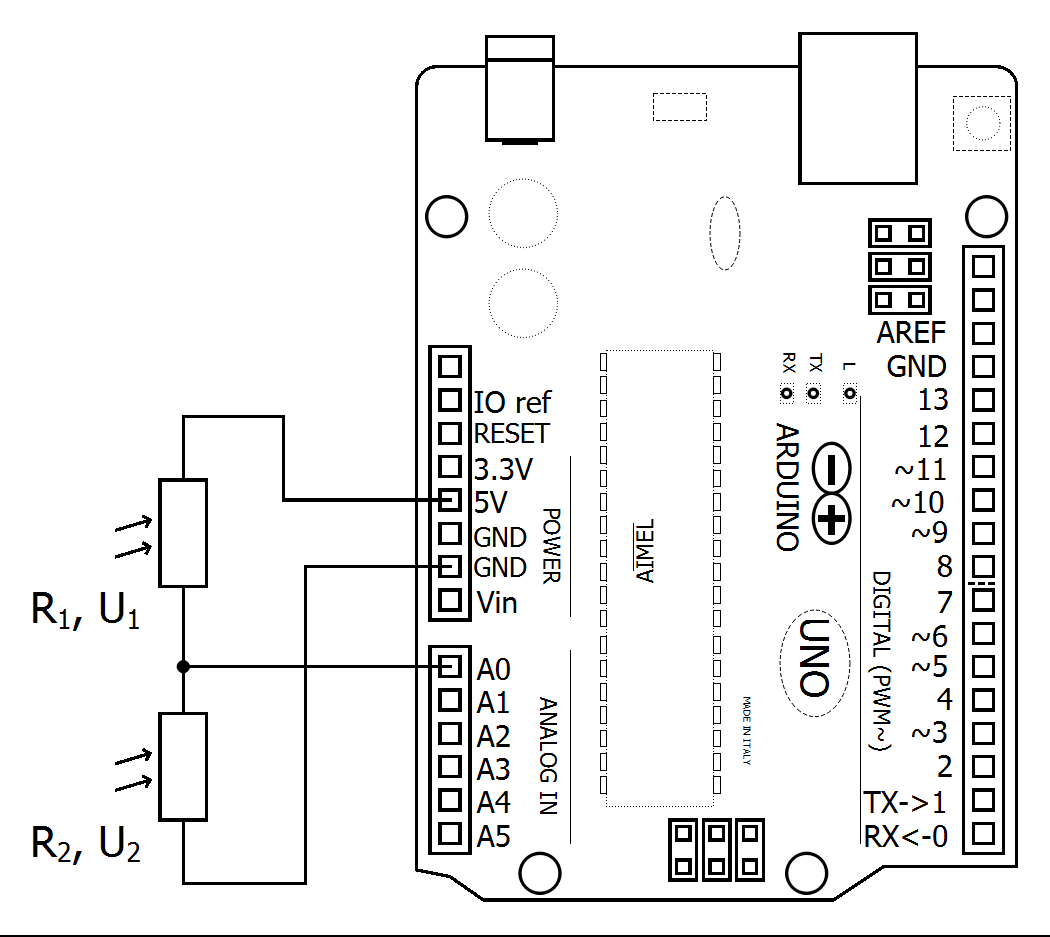
\includegraphics[width=\textwidth]{./Zeichnungen/schaltplan-ldr-in-reihe.png}
	\end{minipage}

	\begin{enumerate}[label=\alph*), itemsep=0mm, parsep=0mm]
		\setcounter{enumi}{2}
		\item Entwickle mithilfe der unten abgebildeten Befehle ein Programm, das auf dem seriellen Monitor ausgibt, welches Moorhuhn (welcher LDR) getroffen wurde. Das Programm soll als Struktogramm dargestellt werden.
	\end{enumerate}
	
	\begin{figure}[H]
		\centering
		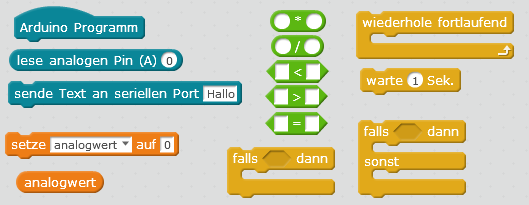
\includegraphics[width=0.8\textwidth]{./pics/befehle-fuer-ldr-in-reihe.png}
	\end{figure}
\end{aufgabe}

\newpage
\begin{aufgabe} \emph{Transistor}
	
	\begin{wrapfigure}{r}{0.4\textwidth}
		\centering
		\vspace{-\baselineskip}
		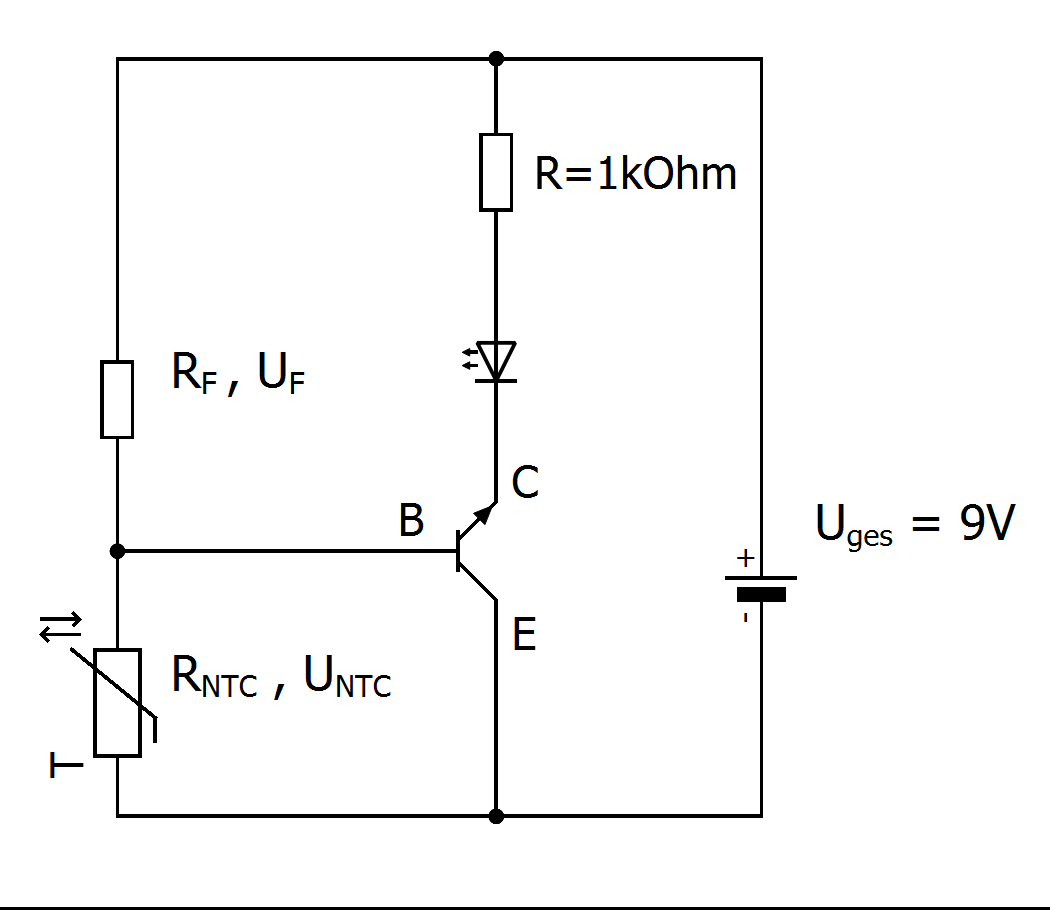
\includegraphics[width=0.4\textwidth]{./Zeichnungen/schaltplan-transistor-und-ntc.png}
	\end{wrapfigure}
	Der Schaltplan rechts zeigt eine Transistor-Grundschaltung, in der ein Spannungsteiler mit einem Festwiderstand $R_F$ und ein NTC mit Widerstand $R_{NTC}$ verbaut ist. In der folgenden Tabelle ist festgehalten, bei welcher Temperatur der NTC welchen Widerstand hat.
	
	\medskip
	\begin{tabular}{l|l|l|l}
		$T$ in $\SI{}{\celsius}$ & 25 & 20 & 15 \\ \hline
		$R$ in $\SI{}{\kilo\ohm}$ & 10 & 12,1 & 14,8 \\
	\end{tabular}
	
	\medskip
	Bestimme die Größe von $R_F$ so, dass der Transistor bei $\SI{25}{\celsius}$ ($\SI{20}{\celsius}$, $\SI{15}{\celsius}$) schaltet.
	
	\emph{Hinweis:} Der Transistor schaltet bei einer Spannung $U_{BE} = \SI{0,7}{\volt}$.
\end{aufgabe}

\vfill
\begin{links}
	\item \href{https://www.instructables.com/id/Arduino-UNO-Laser-Game/}{Laser-Game}
	
	Ein kleines Spiel, das sich auf einfache Weise nachbauen lässt.
	
	\item \href{https://www.youtube.com/watch?v=O_Q1WKCtWiA}{Arduino Garden Controller}
	
	Gartenarbeit muss heute nicht mehr aufwendig sein: Mit einem Arduino lassen sich die Pflanzen automatisch bewässern, wenn die Erde nicht mehr feucht genug ist. Die erhobenen Daten lassen sich außerdem schön visualisieren.
	
	\item \href{https://www.youtube.com/watch?v=at7wmm9t8UE}{Wetterstation von bitluni}
	
	\href{https://www.youtube.com/watch?v=aHkec8bA8iI}{Das Problem mit Wettervorhersagen (\emph{Dr. Whatson}, Youtube)}
	
	Selbst gebaute Wetterstationen sind beliebte Anfängerprojekte, bei denen meist ein WLAN-fähiger Mikrocontroller auf Basis des ESP8266 zum Einsatz kommt. Dieser lässt sich ebenfalls über die Arduino IDE programmieren. Wer etwas mehr Hintergrundwissen dazu haben will, schaut sich das Video von \emph{Dr. Whatson} an, der außerdem das Projekt \href{https://www.sensebox.de/}{SenseBox} vorstellt.
	
	\item \href{https://www.youtube.com/watch?v=KtSCo6hIlRQ}{\enquote{Use the force or your brainwaves} (Youtube)}
	
	\href{https://create.arduino.cc/projecthub/Imetomi/use-the-force-or-your-brainwaves-9e839b}{\enquote{Use the force or your brainwaves} (Projektseite)}
		
	Der Schüler Imets Tamás hat es mithilfe mehrerer Arduinos geschafft, seine Gehirnwellen einzulesen und zu nutzen, um einen Roboter zu steuern!
\end{links}